% Options for packages loaded elsewhere
\PassOptionsToPackage{unicode}{hyperref}
\PassOptionsToPackage{hyphens}{url}
%
\documentclass[
  english,
  man,floatsintext]{apa6}
\usepackage{amsmath,amssymb}
\usepackage{lmodern}
\usepackage{iftex}
\ifPDFTeX
  \usepackage[T1]{fontenc}
  \usepackage[utf8]{inputenc}
  \usepackage{textcomp} % provide euro and other symbols
\else % if luatex or xetex
  \usepackage{unicode-math}
  \defaultfontfeatures{Scale=MatchLowercase}
  \defaultfontfeatures[\rmfamily]{Ligatures=TeX,Scale=1}
\fi
% Use upquote if available, for straight quotes in verbatim environments
\IfFileExists{upquote.sty}{\usepackage{upquote}}{}
\IfFileExists{microtype.sty}{% use microtype if available
  \usepackage[]{microtype}
  \UseMicrotypeSet[protrusion]{basicmath} % disable protrusion for tt fonts
}{}
\makeatletter
\@ifundefined{KOMAClassName}{% if non-KOMA class
  \IfFileExists{parskip.sty}{%
    \usepackage{parskip}
  }{% else
    \setlength{\parindent}{0pt}
    \setlength{\parskip}{6pt plus 2pt minus 1pt}}
}{% if KOMA class
  \KOMAoptions{parskip=half}}
\makeatother
\usepackage{xcolor}
\IfFileExists{xurl.sty}{\usepackage{xurl}}{} % add URL line breaks if available
\IfFileExists{bookmark.sty}{\usepackage{bookmark}}{\usepackage{hyperref}}
\hypersetup{
  pdftitle={The Sound of Teaching Music: Expert Pianists' Performance Modulations for Novices},
  pdfauthor={Atsuko Tominaga1, Günther Knoblich1, \& Natalie Sebanz1},
  pdflang={en-EN},
  pdfkeywords={teaching, expertise, skill transmission, artistic expression, music},
  hidelinks,
  pdfcreator={LaTeX via pandoc}}
\urlstyle{same} % disable monospaced font for URLs
\usepackage{graphicx}
\makeatletter
\def\maxwidth{\ifdim\Gin@nat@width>\linewidth\linewidth\else\Gin@nat@width\fi}
\def\maxheight{\ifdim\Gin@nat@height>\textheight\textheight\else\Gin@nat@height\fi}
\makeatother
% Scale images if necessary, so that they will not overflow the page
% margins by default, and it is still possible to overwrite the defaults
% using explicit options in \includegraphics[width, height, ...]{}
\setkeys{Gin}{width=\maxwidth,height=\maxheight,keepaspectratio}
% Set default figure placement to htbp
\makeatletter
\def\fps@figure{htbp}
\makeatother
\setlength{\emergencystretch}{3em} % prevent overfull lines
\providecommand{\tightlist}{%
  \setlength{\itemsep}{0pt}\setlength{\parskip}{0pt}}
\setcounter{secnumdepth}{-\maxdimen} % remove section numbering
% Make \paragraph and \subparagraph free-standing
\ifx\paragraph\undefined\else
  \let\oldparagraph\paragraph
  \renewcommand{\paragraph}[1]{\oldparagraph{#1}\mbox{}}
\fi
\ifx\subparagraph\undefined\else
  \let\oldsubparagraph\subparagraph
  \renewcommand{\subparagraph}[1]{\oldsubparagraph{#1}\mbox{}}
\fi
% Manuscript styling
\usepackage{upgreek}
\captionsetup{font=singlespacing,justification=justified}

% Table formatting
\usepackage{longtable}
\usepackage{lscape}
% \usepackage[counterclockwise]{rotating}   % Landscape page setup for large tables
\usepackage{multirow}		% Table styling
\usepackage{tabularx}		% Control Column width
\usepackage[flushleft]{threeparttable}	% Allows for three part tables with a specified notes section
\usepackage{threeparttablex}            % Lets threeparttable work with longtable

% Create new environments so endfloat can handle them
% \newenvironment{ltable}
%   {\begin{landscape}\begin{center}\begin{threeparttable}}
%   {\end{threeparttable}\end{center}\end{landscape}}
\newenvironment{lltable}{\begin{landscape}\begin{center}\begin{ThreePartTable}}{\end{ThreePartTable}\end{center}\end{landscape}}

% Enables adjusting longtable caption width to table width
% Solution found at http://golatex.de/longtable-mit-caption-so-breit-wie-die-tabelle-t15767.html
\makeatletter
\newcommand\LastLTentrywidth{1em}
\newlength\longtablewidth
\setlength{\longtablewidth}{1in}
\newcommand{\getlongtablewidth}{\begingroup \ifcsname LT@\roman{LT@tables}\endcsname \global\longtablewidth=0pt \renewcommand{\LT@entry}[2]{\global\advance\longtablewidth by ##2\relax\gdef\LastLTentrywidth{##2}}\@nameuse{LT@\roman{LT@tables}} \fi \endgroup}

% \setlength{\parindent}{0.5in}
% \setlength{\parskip}{0pt plus 0pt minus 0pt}

% \usepackage{etoolbox}
\makeatletter
\patchcmd{\HyOrg@maketitle}
  {\section{\normalfont\normalsize\abstractname}}
  {\section*{\normalfont\normalsize\abstractname}}
  {}{\typeout{Failed to patch abstract.}}
\patchcmd{\HyOrg@maketitle}
  {\section{\protect\normalfont{\@title}}}
  {\section*{\protect\normalfont{\@title}}}
  {}{\typeout{Failed to patch title.}}
\makeatother
\shorttitle{The Sound of Teaching Music}
\keywords{teaching, expertise, skill transmission, artistic expression, music\newline\indent Word count: around 5500 (except references)}
\usepackage{csquotes}
\ifXeTeX
  % Load polyglossia as late as possible: uses bidi with RTL langages (e.g. Hebrew, Arabic)
  \usepackage{polyglossia}
  \setmainlanguage[]{english}
\else
  \usepackage[main=english]{babel}
% get rid of language-specific shorthands (see #6817):
\let\LanguageShortHands\languageshorthands
\def\languageshorthands#1{}
\fi
\ifLuaTeX
  \usepackage{selnolig}  % disable illegal ligatures
\fi
\newlength{\cslhangindent}
\setlength{\cslhangindent}{1.5em}
\newlength{\csllabelwidth}
\setlength{\csllabelwidth}{3em}
\newenvironment{CSLReferences}[2] % #1 hanging-ident, #2 entry spacing
 {% don't indent paragraphs
  \setlength{\parindent}{0pt}
  % turn on hanging indent if param 1 is 1
  \ifodd #1 \everypar{\setlength{\hangindent}{\cslhangindent}}\ignorespaces\fi
  % set entry spacing
  \ifnum #2 > 0
  \setlength{\parskip}{#2\baselineskip}
  \fi
 }%
 {}
\usepackage{calc}
\newcommand{\CSLBlock}[1]{#1\hfill\break}
\newcommand{\CSLLeftMargin}[1]{\parbox[t]{\csllabelwidth}{#1}}
\newcommand{\CSLRightInline}[1]{\parbox[t]{\linewidth - \csllabelwidth}{#1}\break}
\newcommand{\CSLIndent}[1]{\hspace{\cslhangindent}#1}

\title{The Sound of Teaching Music: Expert Pianists' Performance Modulations for Novices}
\author{Atsuko Tominaga\textsuperscript{1}, Günther Knoblich\textsuperscript{1}, \& Natalie Sebanz\textsuperscript{1}}
\date{}


\authornote{

Correspondence concerning this article should be addressed to Atsuko Tominaga, Quellenstraße 51, 1100 Vienna, Austria. E-mail: \href{mailto:Tominaga_Atsuko@phd.ceu.edu}{\nolinkurl{Tominaga\_Atsuko@phd.ceu.edu}}

}

\affiliation{\vspace{0.5cm}\textsuperscript{1} Department of Cognitive Science, Central European University}

\abstract{
Experts modulate their performance of actions for teaching purposes, performing slower and exaggerated movements when demonstrating novel actions to novices. The present study asked whether such modulations are also used to teach techniques of artistic expression. One domain where subtle movement modulations are crucial for achieving artistic expression is music. We investigated how skilled pianists modulate their playing to demonstrate to students the techniques required for conveying piece-related musical expressions, compared to performing the piece without didactic intentions. Expressions in the piece concerned either articulation (i.e., legato and staccato) or dynamics (i.e., forte and piano). The pianists played either with the goal to perform the piece to an audience or with the goal to teach the respective techniques to novices. When intending to teach articulation, skilled pianists produced more exaggerated staccato. When intending to teach dynamics, they created a larger contrast between forte and piano at structurally important points. We found consistent results with a simple musical scale (Experiment 1) and a more naturalistic piece of music (Experiment 2). These findings suggest that action modulations are performed not only to attract learners' attention but to highlight the most relevant aspects of the actions to be learnt.
}



\begin{document}
\maketitle

\hypertarget{introduction}{%
\section{1. Introduction}\label{introduction}}

Deliberate teaching has supported human skill transmission over generations and provides a key route for learning (Thornton \& Raihani, 2008; Tomasello, 2016). Experts modulate their behaviour so that novices can extract relevant information to learn a novel skill. In particular, adults modulate their speech (motherese) and actions (motionese) when demonstrating a skill to infant learners (Brand, Baldwin, \& Ashburn, 2002; Saint-Georges et al., 2013). These modulations include slowing down and exaggerating sounds and actions. Similar findings were obtained in studies with adult learners, where exaggerations were observed when native British English speakers were talking to first language English learners (Uther, Knoll, \& Burnham, 2007) and when skilled adults were teaching xylophone melodies to novices (McEllin, Knoblich, \& Sebanz, 2017). The observed modulations are thought to provide communicative signals that can facilitate learning by affecting attention and memory (Csibra \& Gergely, 2009).

Previous research has shown that demonstrators not only adjust their gestures (Campisi \& Özyürek, 2013) and actions (Fukuyama et al., 2015) to learners' skills but engage in specific action modulations to highlight particular aspects of demonstrated actions. For example, Schaik, Meyer, Ham, and Hunnius (2019) showed that adults used specific action modulations for demonstrating different action effects of objects to infants. Ho, Littman, MacGlashan, Cushman, and Austerweil (2016) found that demonstrators chose costly movement paths at structurally important points to disambiguate one goal over other possibilities.

Importantly, in some domains teaching requires not only demonstrating \emph{what} to do, but \emph{how} to perform actions. In artistic contexts, novices need to learn how exactly to perform actions by relying on particular techniques (Sloboda, 2000). For example, when playing a piece of music on the piano, it is not sufficient to press the keys in the correct order, but learners need to be able to implement expressive techniques (Juslin, 2003). This raises the question of whether and how experts modulate their actions during didactic demonstration in artistic contexts, where expressivity is an integral part of what learners need to acquire. Studying action modulations that serve the teaching of artistic techniques is also of broader theoretical importance: It can show whether action modulations can be used to selectively highlight subtle aspects of actions that define expert performance.

In the present study, we employed musical expressive techniques as skills to be taught because multiple properties of the performance (e.g., timing, smoothness, loudness) can be modulated at the same time. Specific and subtle aspects of the performance may need to be highlighted to teach a respective technique. Pianists were asked to perform a piece in order to demonstrate to a learner how to implement the notated expressions (teaching condition) and to play the same piece for an audience (performing condition). Two basic expressive techniques in piano performance were used: articulation (legato and staccato) and dynamics (forte and piano).

If experts rely on generic action modulations, it can be expected that they will play more slowly during didactic demonstration, regardless of the kind of expressive techniques to be taught. To the extent that experts use action modulations to support their teaching of specific expressive techniques, they should produce longer legato and shorter staccato when teaching articulation whereas they should produce louder forte and softer piano when teaching dynamics. Furthermore, one could speculate that they might produce modulations specifically at structurally important points that best highlight the technique to be taught. Importantly, they should avoid modulating irrelevant properties of expression, e.g., the smoothness of sound while teaching dynamics.

In Experiment 1, we employed a simple musical scale to examine whether and how skilled pianists vary their performance depending on which expressive techniques (i.e., either articulation or dynamics) they are teaching. Experiment 2 was conducted to replicate our findings from Experiment 1 with a more naturalistic piece of music.

\hypertarget{experiment-1}{%
\section{2. Experiment 1}\label{experiment-1}}

\hypertarget{method}{%
\subsection{2.1. Method}\label{method}}

\hypertarget{participants}{%
\subsubsection{2.1.1. Participants}\label{participants}}

We recruited 36 piano experts who played the piano for at least the past 10 years or were studying advanced piano performance at a music school at the time of recruitment. For data analysis, we excluded three participants due to experimental errors, and two participants because they deviated substantially from the prescribed tempo (outside 2 standard deviations from the average tempo across participants). Thirty-one participants (15 female) were included in data analysis. Most participants were right-handed (left: 2, ambidextrous: 2) with a mean age of 24.16 (\emph{SD} = 4.26). They had 12.45 years of practice on average (\emph{SD} = 5.66). All participants gave their informed consent before the experiment started and received vouchers for their participation. The study was approved by the United Ethical Review Committee for Research in Psychology (EPKEB) in Hungary.

\hypertarget{apparatus-and-stimuli}{%
\subsubsection{2.1.2. Apparatus and stimuli}\label{apparatus-and-stimuli}}

A weighted Yamaha MIDI digital piano was used to record participants' performance via Max/MSP (\url{https://cycling74.com/products/max}) on a MacBook Pro with Mac OS X Mojave 10.14.3. The laptop and piano were connected to a high-fidelity soundcard (Focusrite Scarlett 6i6) to deliver a metronome and piano sound. All auditory feedback was given to participants through headphones (Audio-Technica ATH-M50X). Sheet music was displayed on a computer monitor in front of the participants. The pitch, onset and offset time of each note, and key velocity profiles were obtained from MIDI data using Max/MSP patchers.

One musical excerpt was used as a stimulus. The excerpt was taken from ``A Dozen a Day - Play with Ease in Many Keys" by Edna-Mae Burnam and modified for the experiment. It consisted of a 6-measure isochronous melody noted in 4/4 meter. The stimulus was composed in C major to be played with the right hand only. Non-expressive sheet music (i.e., sheet music without expressive notations, \emph{Figure \ref{fig:stimuli}, A}) was used for the purpose of practice. Expressive notations were added to the non-expressive sheet music for the experiment. They referred to either articulation or dynamics (\emph{Figure \ref{fig:stimuli}, B-C}). Articulation was notated as either legato or staccato. Legato indicates that musical notes are to be connected and should sound smooth. Staccato requires producing musical notes with shortened duration, keeping them separate from each other. Dynamics was notated as either forte and piano. Forte indicates that musical notes should be played loudly whereas piano indicates that musical notes should be played softly. The notation did not include any indication of fingering (i.e., the positioning of the fingers when playing the piano) because the piece was simple and pilot testing had shown that specifying fingering was not necessary.

\hypertarget{procedure}{%
\subsubsection{2.1.3. Procedure}\label{procedure}}

First, participants were allocated to either the teaching or performing condition and asked to practise the excerpt with the notated expression of either articulation or dynamics (\emph{Figure \ref{fig:stimuli}, B-C}). As soon as they had produced the excerpt with the notated expression without pitch errors twice consecutively, the test trials began.

In the teaching condition, participants were instructed to play the excerpt of music as if they were teaching it to students. It was mentioned that the students already knew the sequence of the tones and that they were trying to learn how to perform the piece with the notated expression by listening to the participant's performance. In the performing condition, participants were asked to play the excerpt of music as if they were performing it to an audience (see details in \emph{\protect\hyperlink{supplementary}{Supplementary Materials}}). Participants played the piece 8 times per expressive technique per condition, so there were 32 trials in total (2 conditions x 2 expressive techniques x 8 trials). The order of the conditions was blocked and counterbalanced across participants. The order of the expressive techniques within each condition was also blocked and counterbalanced across participants. A leading metronome (80 quarter-beats per minute, 8 beats) indicated the target tempo before each trial.

At the end of the experiment, participants filled in a questionnaire asking about their demographic information and experience in piano performance/teaching.

\hypertarget{data-analysis}{%
\subsubsection{2.1.4. Data analysis}\label{data-analysis}}

Three dependent variables were computed for data analysis. Interonset intervals (IOIs) are the intervals between onsets of adjacent notes and provide a measure of tempo. Key-overlap time (KOT) is the difference between the offset time of the current tone (i.e., key release time) and the onset time of the ensuing tone, and measures the smoothness of musical sequences (Bresin \& Battel, 2000). A positive value indicates smooth legato styles due to overlap between the current and ensuing tone whereas a negative value indicates sharp staccato styles due to separation between the current and ensuing tone. Tone intensity is assessed by key velocity (KV) and measures the loudness of a musical note. The value of KV in MIDI varies between 0 (minimum) and 127 (maximum).

Data cleaning, preprocessing and statistical analysis were performed in R version 4.0.5. For statistical analysis, only 16th notes with expressive notations were included. Overall, five trials were excluded from data analysis because participants did not follow the sheet music or stopped performing before the end. Pitch errors were identified by comparing the sequence of musical notes produced by a participant with the sequence of musical notes according to the sheet music. Pitch errors included either extra, missing or substituted tones and were manually removed by using the \emph{editData} R package. For onsets, 11.65\% of the trials contained at least one pitch error (extra notes: 6.28\%, missing notes: 5.07\%, substituted notes: 0.30\%). For offsets, 14.08\% of the trials contained at least one pitch error (extra notes: 6.28\%, missing notes: 5.17\%, substituted notes: 2.63\%). As a result, less than 1 \% of total responses were corrected. In addition to pitch errors, we removed outliers for IOIs, KOT and KV, defined as values more than 3 standard deviations from the mean of each dependent variable and excluded from data analysis. For each dependent variable, this resulted in less than 5\% of overall responses being removed as outliers.

We performed separate analyses for the two expressive techniques (i.e., articulation, dynamics). A paired-sample \emph{t}-test or a Wilcoxon Signed-rank test (a non-parametric alternative to a paired \emph{t}-test) was performed to compare the mean IOIs in the teaching and performing condition. For KOT and KV, we performed a 2 x 2 repeated-measures analysis of variance (ANOVA) with the factors Condition (teaching vs.~performing) and Subcomponent (LS: legato vs.~staccato or FP: forte vs.~piano, respectively). The \emph{t.test} or \emph{wilcox.test} function in the \emph{stats} R package was used for a \emph{t}-test or a Wilcoxon Signed-rank test. For calculating an effect size, we used the \emph{rstatix} R package. The \emph{aov\_car} function in the \emph{afex} R package was used for a repeated-measures ANOVA. For post-hoc comparisons on the estimated marginal means, we used the \emph{emmeans} R package.

\begin{figure}
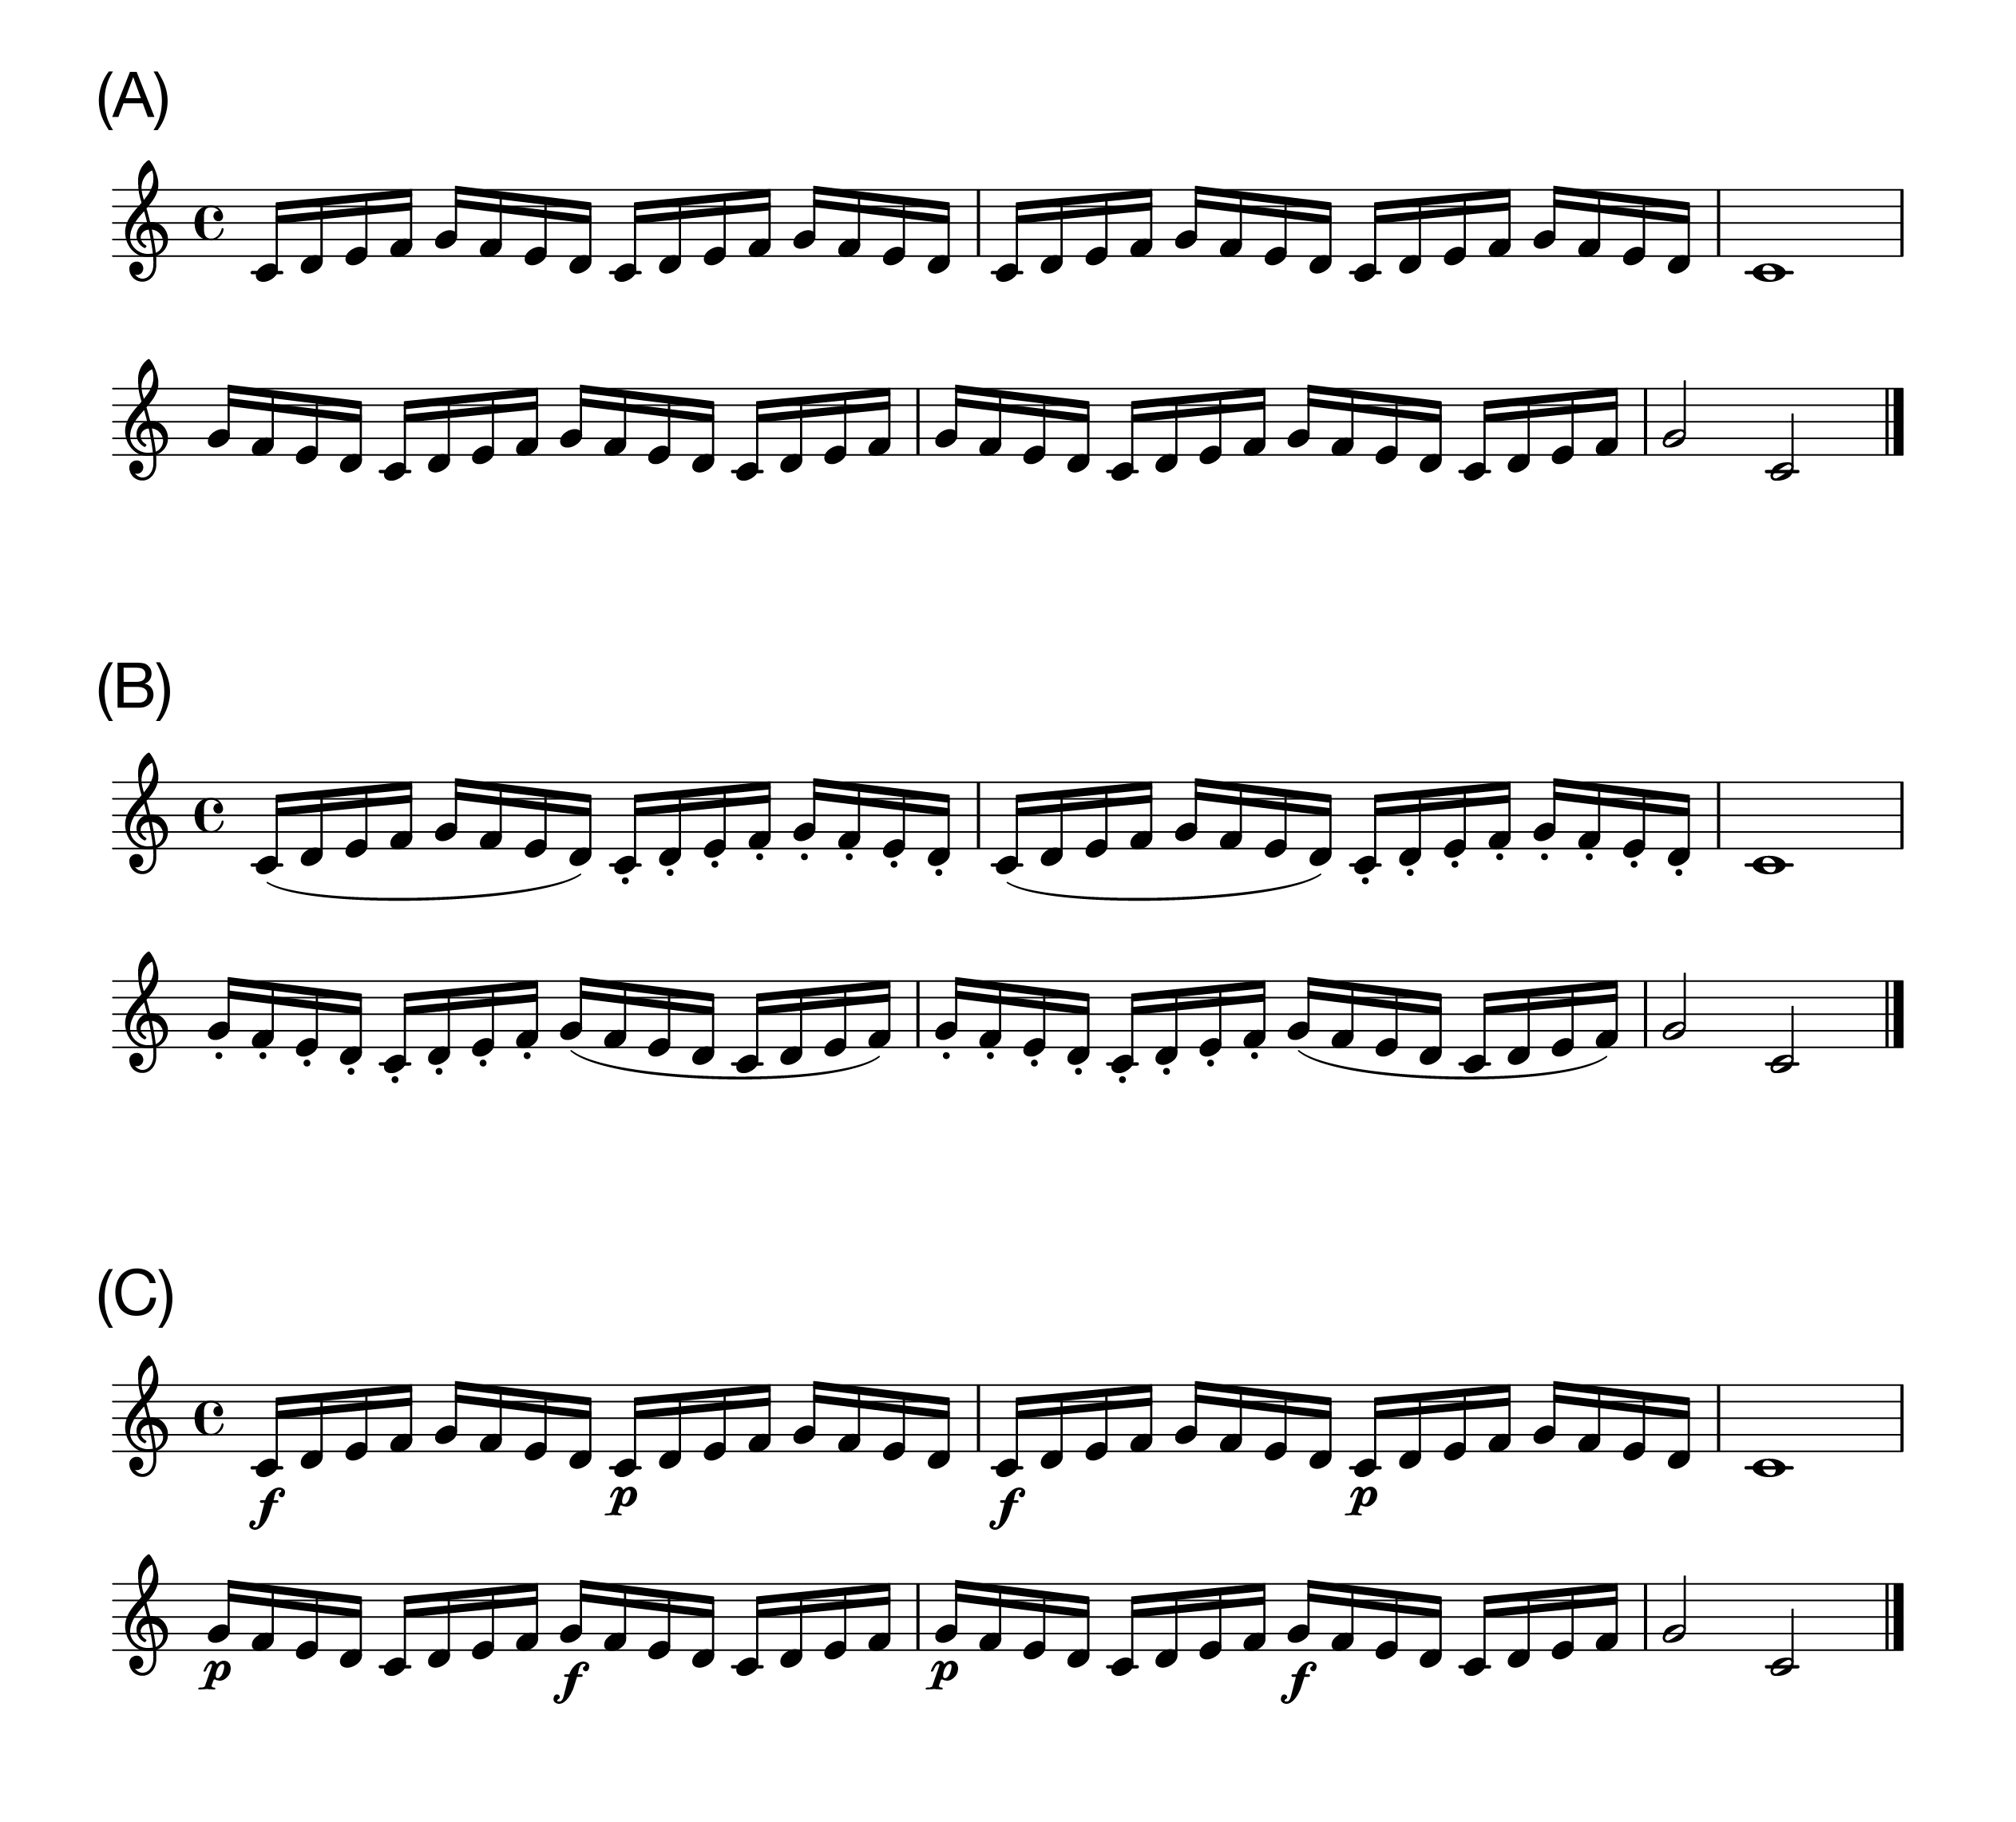
\includegraphics[width=1\linewidth]{manuscript_files/figure-latex/stim-1-1} \caption{\label{fig:stimuli}(A)Non-expressive sheet music. (B)Articulation. The curved line (slur) indicates legato and the dots indicate staccato. (C)Dynamics. The symbol `f' denotes forte and the symbol `p' denotes piano. For data analysis, only the 16th notes were included.}\label{fig:stim-1}
\end{figure}

\newpage

\hypertarget{results}{%
\subsection{2.2. Results}\label{results}}

All effects are reported as significant at \emph{p} \textless{} .05. We first report results for performance of the piece with the notated expression of articulation (\emph{Figure \ref{fig:stimuli}, B}), followed by performance of the piece with the notated expression of dynamics (\emph{Figure \ref{fig:stimuli}, C}). To recall our predictions, if participants play more slowly when they are trying to teach, interonset intervals (IOIs) should be larger when teaching. If participants specifically modulate relevant aspects of the expressive techniques they are trying to teach, key-overlap time (KOT) should reveal exaggerated legato/staccato when teaching articulation, and key velocity (KV) should reveal amplifications of forte and piano when teaching dynamics.

\hypertarget{articulation-interonset-intervals-iois}{%
\subsubsection{2.2.1. Articulation: Interonset Intervals (IOIs)}\label{articulation-interonset-intervals-iois}}

In order to compare the mean IOIs between the teaching and performing condition, we conducted a Wiscoxon Signed-rank test, instead of a paired \emph{t}-test, because a Shapiro-Wilk test showed that the distribution of the mean difference was significantly different from the normal distribution (\emph{p} \textless{} 0.001). The Wiscoxon Signed-rank test revealed that participants played more slowly in the teaching condition {[}\emph{Mdn} = 189.55 (ms), \emph{IQR} = 26.74{]} than in the performing condition {[}\emph{Mdn} = 185.24 (ms), \emph{IQR} = 19.32{]} while playing the piece with the notated articulation (\emph{p} = 0.021, \emph{r} = 0.41, \emph{Figure \ref{fig:ioi-1}}).

\hypertarget{articulation-key-overlap-time-kot}{%
\subsubsection{2.2.2. Articulation: Key-Overlap Time (KOT)}\label{articulation-key-overlap-time-kot}}

A two-way repeated-measures ANOVA with the factors Condition (teaching vs.~performing) and Subcomponent-LS (legato vs.~staccato) revealed that there was a significant main effect of Subcomponent-LS (\emph{F}(1,30) = 1158, \emph{p} \textless{} 0.001, \(\eta_G^2\) = 0.94) and a significant interaction between Condition and Subcomponent-LS (\emph{F}(1,30) = 8.31, \emph{p} = 0.007, \(\eta_G^2\) = 0.011, \emph{Figure \ref{fig:kot-1}}). Post-hoc comparisons based on the estimated marginal means with Tukey adjustment showed that participants produced shorter staccato in the teaching condition {[}\emph{M} = -134.03 (ms), \emph{SD} = 19.86{]} than in the performing condition {[}\emph{M} = -128.35 (ms), \emph{SD} = 20.80{]} (\emph{p} = 0.004) while there was no significant difference in legato between the teaching {[}\emph{M} = 15.91 (ms), \emph{SD} = 15.49{]} and performing condition {[}\emph{M} = 14.00 (ms), \emph{SD} = 17.01{]} (\emph{p} = 0.32).

\hypertarget{articulation-key-velocity-kv}{%
\subsubsection{2.2.3. Articulation: Key Velocity (KV)}\label{articulation-key-velocity-kv}}

A two-way repeated-measures ANOVA with the factors Condition (teaching vs.~performing) and Subcomponent-LS (legato vs.~staccato) showed that there was a significant interaction between Condition and Subcomponent-LS (\emph{F}(1,30) = 7.38, \emph{p} = 0.011, \(\eta_G^2\) = 0.004, \emph{Figure \ref{fig:vel-1}}). However, post-hoc comparisons based on the estimated marginal means with Tukey adjustment did not find a significant difference between the teaching {[}Legato: \emph{M} = 70.34, \emph{SD} = 6.45; Staccato: \emph{M} = 72.01, \emph{SD} = 8.74{]} and performing condition {[}Legato: \emph{M} = 70.68, \emph{SD} = 5.84, Staccato: \emph{M} = 70.42, \emph{SD} = 7.96{]} for each subcomponent (Legato: \emph{p} = 0.70, Staccato: \emph{p} = 0.07).

\hypertarget{dynamics-interonset-intervals-iois}{%
\subsubsection{2.2.4. Dynamics: Interonset Intervals (IOIs)}\label{dynamics-interonset-intervals-iois}}

In order to compare the mean IOIs between the teaching and performing condition, we conducted a Wiscoxon Signed-rank test, instead of a paired \emph{t}-test, because a Shapiro-Wilk test showed that the distribution of the mean difference was significantly different from the normal distribution (\emph{p} \textless{} 0.001). The Wiscoxon Signed-rank test revealed no significant difference between the teaching condition {[}\emph{Mdn} = 186.29 (ms), \emph{IQR} = 21.83{]} and the performing condition {[}\emph{Mdn} = 186.27 (ms), \emph{IQR} = 19.58{]} while playing the piece with the notated dynamics (\emph{p} = 0.11, \emph{r} = 0.29, \emph{Figure \ref{fig:ioi-1}}).

\hypertarget{dynamics-key-velocity-kv}{%
\subsubsection{2.2.5. Dynamics: Key Velocity (KV)}\label{dynamics-key-velocity-kv}}

A two-way repeated-measures ANOVA with the factors Condition (teaching vs.~performing) and Subcomponent-FP (forte vs.~piano) showed that there was a significant main effect of Subcomponent-FP (\emph{F}(1,30) = 370, \emph{p} \textless{} 0.001, \(\eta_G^2\) = 0.74) and a significant interaction between Condition and Subcomponent-FP (\emph{F}(1,30) = 6.80, \emph{p} = 0.014, \(\eta_G^2\) = 0.003, \emph{Figure \ref{fig:vel-1}}). Post-hoc comparisons based on the estimated marginal means with Tukey adjustment revealed that participants produced louder forte in the teaching condition {[}\emph{M} = 82.78, \emph{SD} = 8.30{]} than in the performing condition {[}\emph{M} = 81.66, \emph{SD} = 7.43{]} (\emph{p} = 0.021) while there was no significant difference in piano between the teaching {[}\emph{M} = 60.63, \emph{SD} = 5.07{]} and performing condition {[}\emph{M} = 60.99, \emph{SD} = 4.40{]} (\emph{p} = 0.45).

\hypertarget{dynamics-kv-transition-points}{%
\subsubsection{2.2.6. Dynamics: KV Transition Points}\label{dynamics-kv-transition-points}}

Additionally, we conducted an exploratory analysis by focusing on specific points at which each subcomponent changed from one to the other (i.e., forte to piano: FtoP, piano to forte: PtoF). These points could be structurally important in order to make a contrast between forte and piano. We calculated the KV difference for each interval by subtracting the KV value of the current note from that of the following note. Outliers were removed using the same criteria as for the other dependent variables and less than 5 \% of the data were excluded from analysis. A two-way repeated-measures ANOVA with the factors Condition (teaching vs.~performing) and Subcomponent-FP (FtoP vs.~PtoF) showed that there was a significant main effect of Subcomponent-FP (\emph{F}(1,30) = 224, \emph{p} \textless{} 0.001, \(\eta_G^2\) = 0.83) and a significant interaction between Condition and Subcomponent-FP (\emph{F}(1,30) = 25.74, \emph{p} \textless{} 0.001, \(\eta_G^2\) = 0.032, \emph{Figure \ref{fig:vel-diff}}). Post-hoc comparisons based on the estimated marginal means with Tukey adjustment showed that there was a larger KV difference when the expressive notation changed from forte to piano (FtoP: \emph{p} = 0.002) and from piano to forte (PtoF: \emph{p} \textless{} 0.001) in the teaching condition {[}FtoP: \emph{M} = -14.06, \emph{SD} = 7.20; PtoF: \emph{M} = 24.26, \emph{SD} = 9.75{]} than in the performing condition {[}FtoP: \emph{M} = -11.69, \emph{SD} = 5.97, PtoF: \emph{M} = 20.88, \emph{SD} = 8.67{]}.

\hypertarget{dynamics-key-overlap-time-kot}{%
\subsubsection{2.2.7. Dynamics: Key-Overlap Time (KOT)}\label{dynamics-key-overlap-time-kot}}

A two-way repeated-measures ANOVA with the factors Condition (teaching vs.~performing) and Subcomponent-FP (forte vs.~piano) revealed that there was a significant main effect of Subcomponent-FP (\emph{F}(1,30) = 377, \emph{p} \textless{} 0.001, \(\eta_G^2\) = 0.31, \emph{Figure \ref{fig:kot-1}}), reflecting more key overlap for forte notes compared to piano notes. Neither the main effect of Condition (\emph{F}(1,30) = 0.42, \emph{p} = 0.52, \(\eta_G^2\) = 0.000) nor the interaction between Condition and Subcomponent-FP (\emph{F}(1,30) = 0.000, \emph{p} = 0.99, \(\eta_G^2\) = 0.000) was significant.

\hypertarget{discussion}{%
\subsection{2.3. Discussion}\label{discussion}}

The findings from Experiment 1 indicated that skilled pianists modified their performance for teaching purposes. For IOIs, we found a small but significant slowing down during teaching specifically when playing the piece with the notated articulation. This finding is in line with earlier studies that found slower performance of actions in a teaching context (e.g., Brand et al., 2002; McEllin et al., 2017). However, we did not find a significant difference in tempo when participants were teaching dynamics. It could be that trying to keep the prescribed tempo (conveyed through the leading metronome) limited the extent to which participants slowed down their performance during teaching. Another possibility is that slower performance may be beneficial to highlight the relation between two notes (i.e., to what extent two notes overlap) and was therefore employed when teaching articulation, whereas slower performance might not help when teaching dynamics.

The results for KOT and KV showed that participants successfully highlighted relevant aspects of articulation and dynamics. Specifically, they produced shorter staccato when teaching articulation and produced louder forte when teaching dynamics. Moreover, our exploratory analysis demonstrated that participants made a larger contrast in dynamics at transition points (i.e., forte to piano or piano to forte). Importantly, participants did not modulate their performance in terms of irrelevant aspects of the techniques for teaching purposes (e.g., modulating the smoothness of sound while teaching dynamics). These findings confirmed that participants modulated their performance in systematic and fine-grained ways in order to teach expressive techniques.

In Experiment 1, we employed a simple musical scale in order to maximise experimental control. To test whether our results generalise to a more naturalistic piece, in Experiment 2, we chose an actual piano piece and modified it for the purpose of the experiment. If pianists selectively highlight the relevant aspects of the techniques to be taught also in a more naturalistic piece containing more opportunities for expression, they should again produce longer legato and shorter staccato while teaching articulation. When teaching dynamics, they should produce louder forte and softer piano. Given the findings we observed in Experiment 1, we also predicted that participants would make a larger contrast between forte and piano at transition points, and that they might play more slowly when teaching, especially when teaching articulation.

\begin{figure}
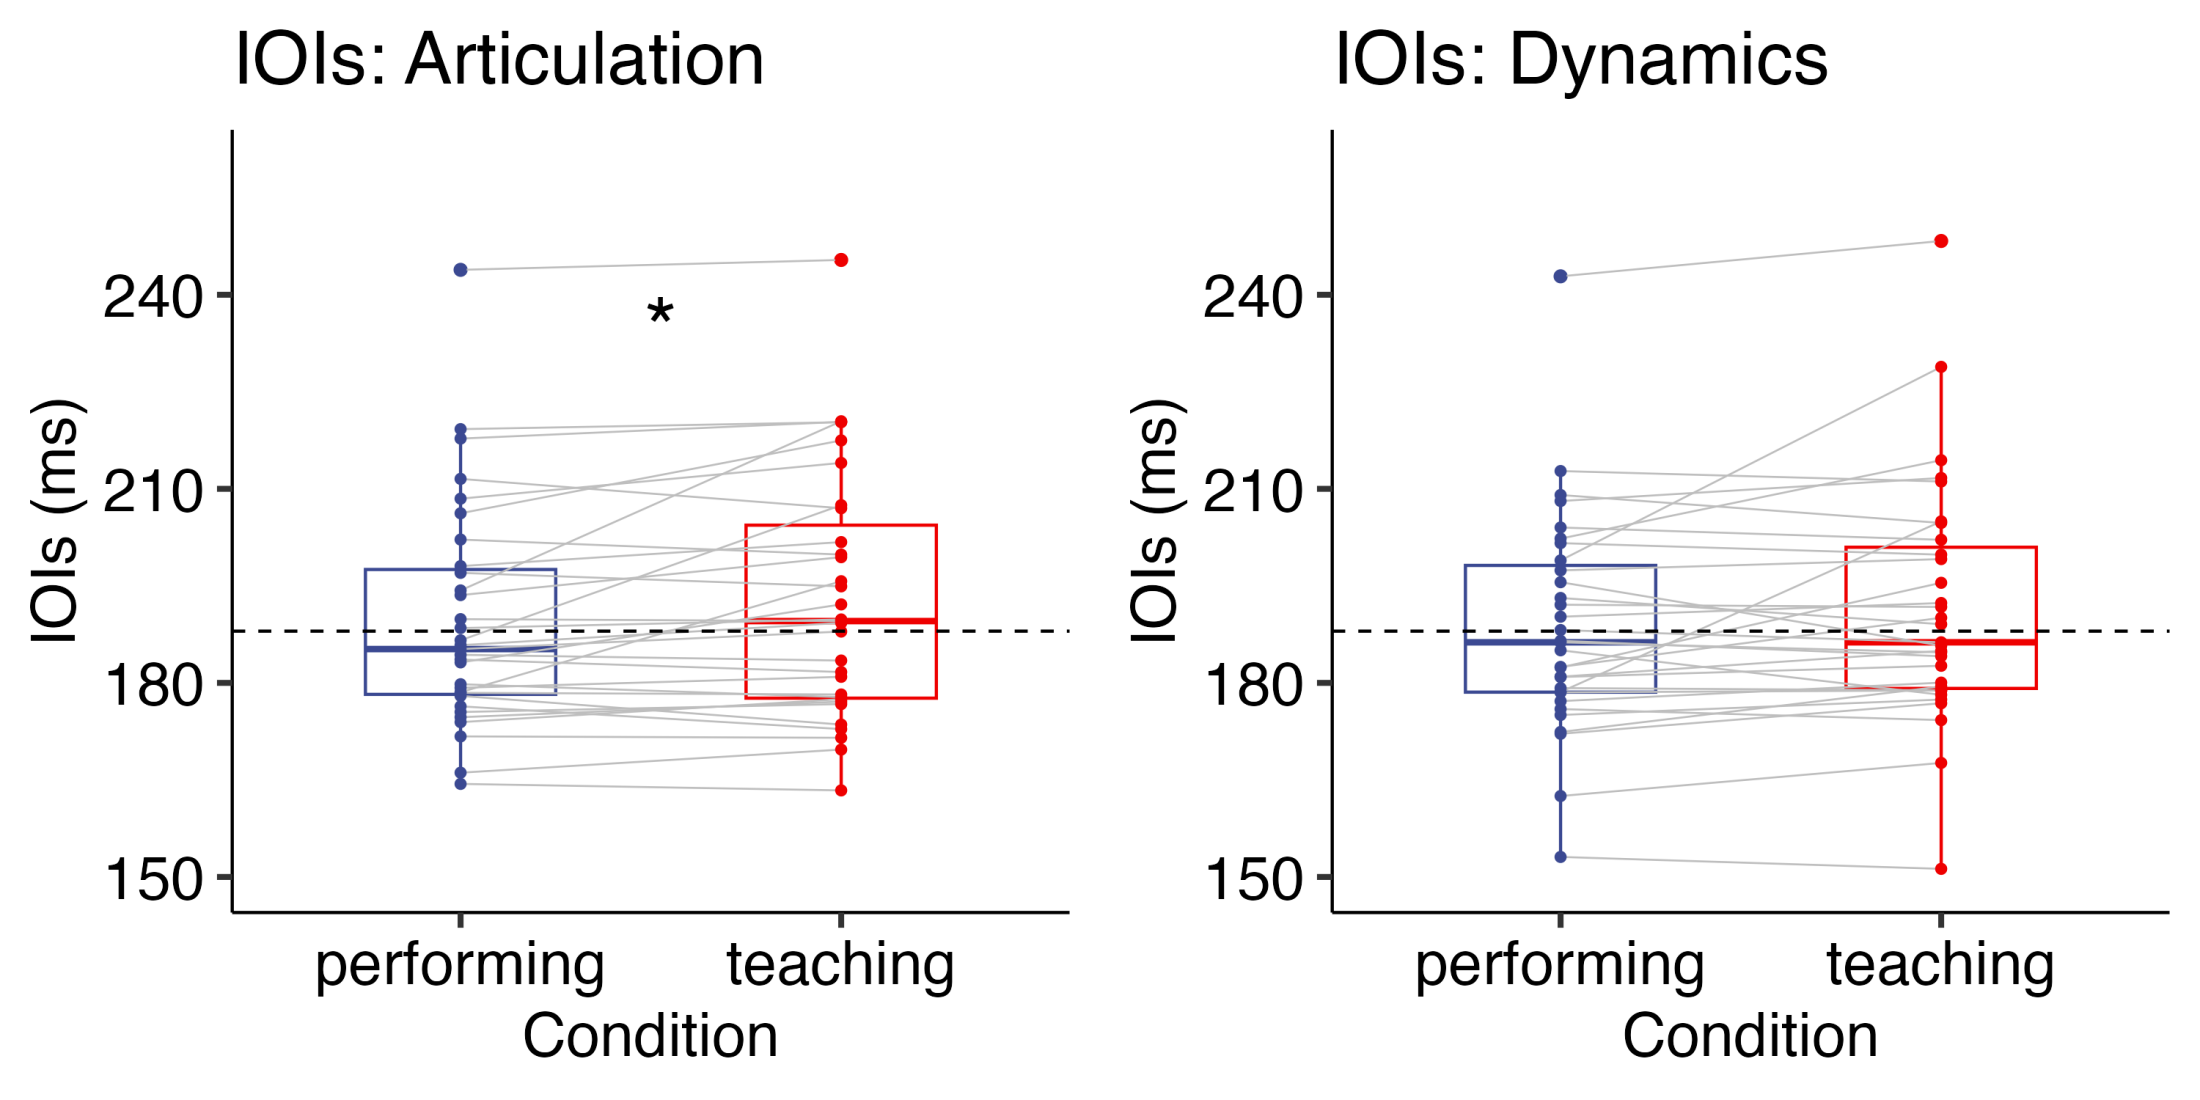
\includegraphics[width=1\linewidth]{manuscript_files/figure-latex/plot-ioi-1-1} \caption{\label{fig:ioi-1}Experiment 1: IOIs (ms) when playing the piece with either articulation (left) or dynamics (right). Each box indicates the IQR with the median, and whiskers extend to a maximum of 1.5 × IQR beyond the box. Significance levels: * \textit{p} < .05, ** \textit{p} < .01, *** \textit{p} < .001}\label{fig:plot-ioi-1}
\end{figure}

\begin{figure}
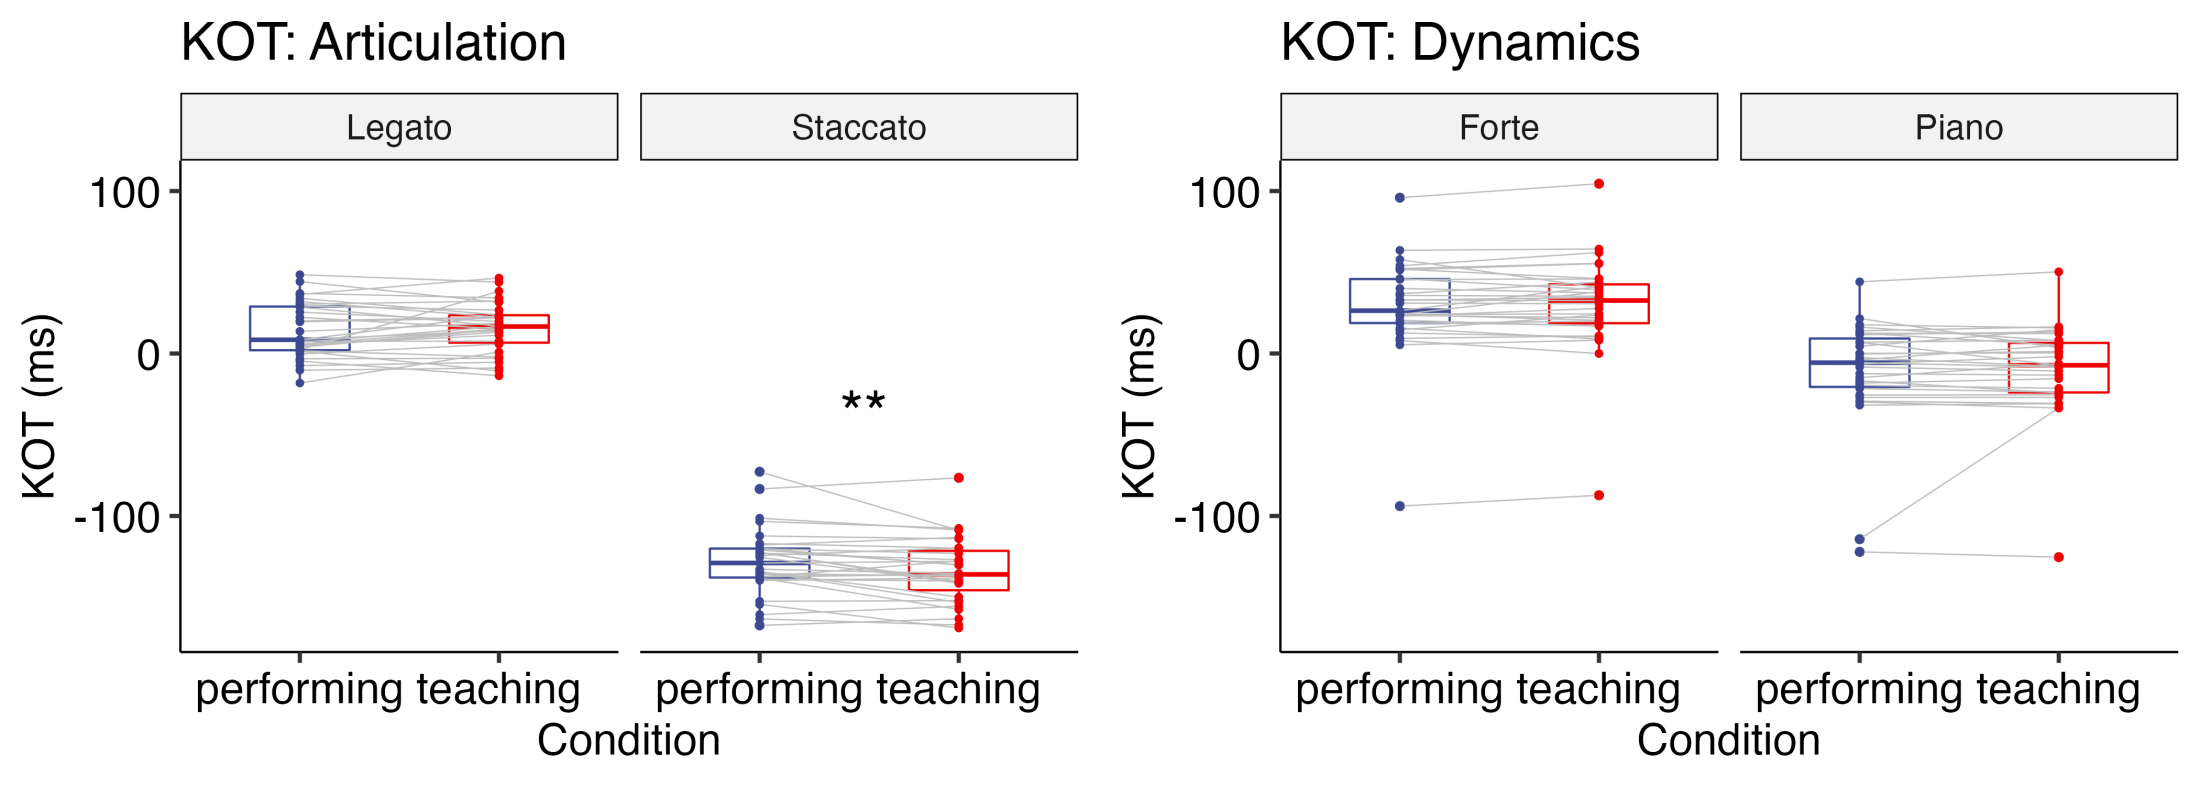
\includegraphics[width=1\linewidth]{manuscript_files/figure-latex/plot-kot-1-1} \caption{\label{fig:kot-1}Experiment 1: KOT (ms) when playing the piece with either articulation (left) or dynamics (right). Each box indicates the IQR with the median, and whiskers extend to a maximum of 1.5 × IQR beyond the box. Significance levels: * \textit{p} < .05, ** \textit{p} < .01, *** \textit{p} < .001}\label{fig:plot-kot-1}
\end{figure}

\begin{figure}
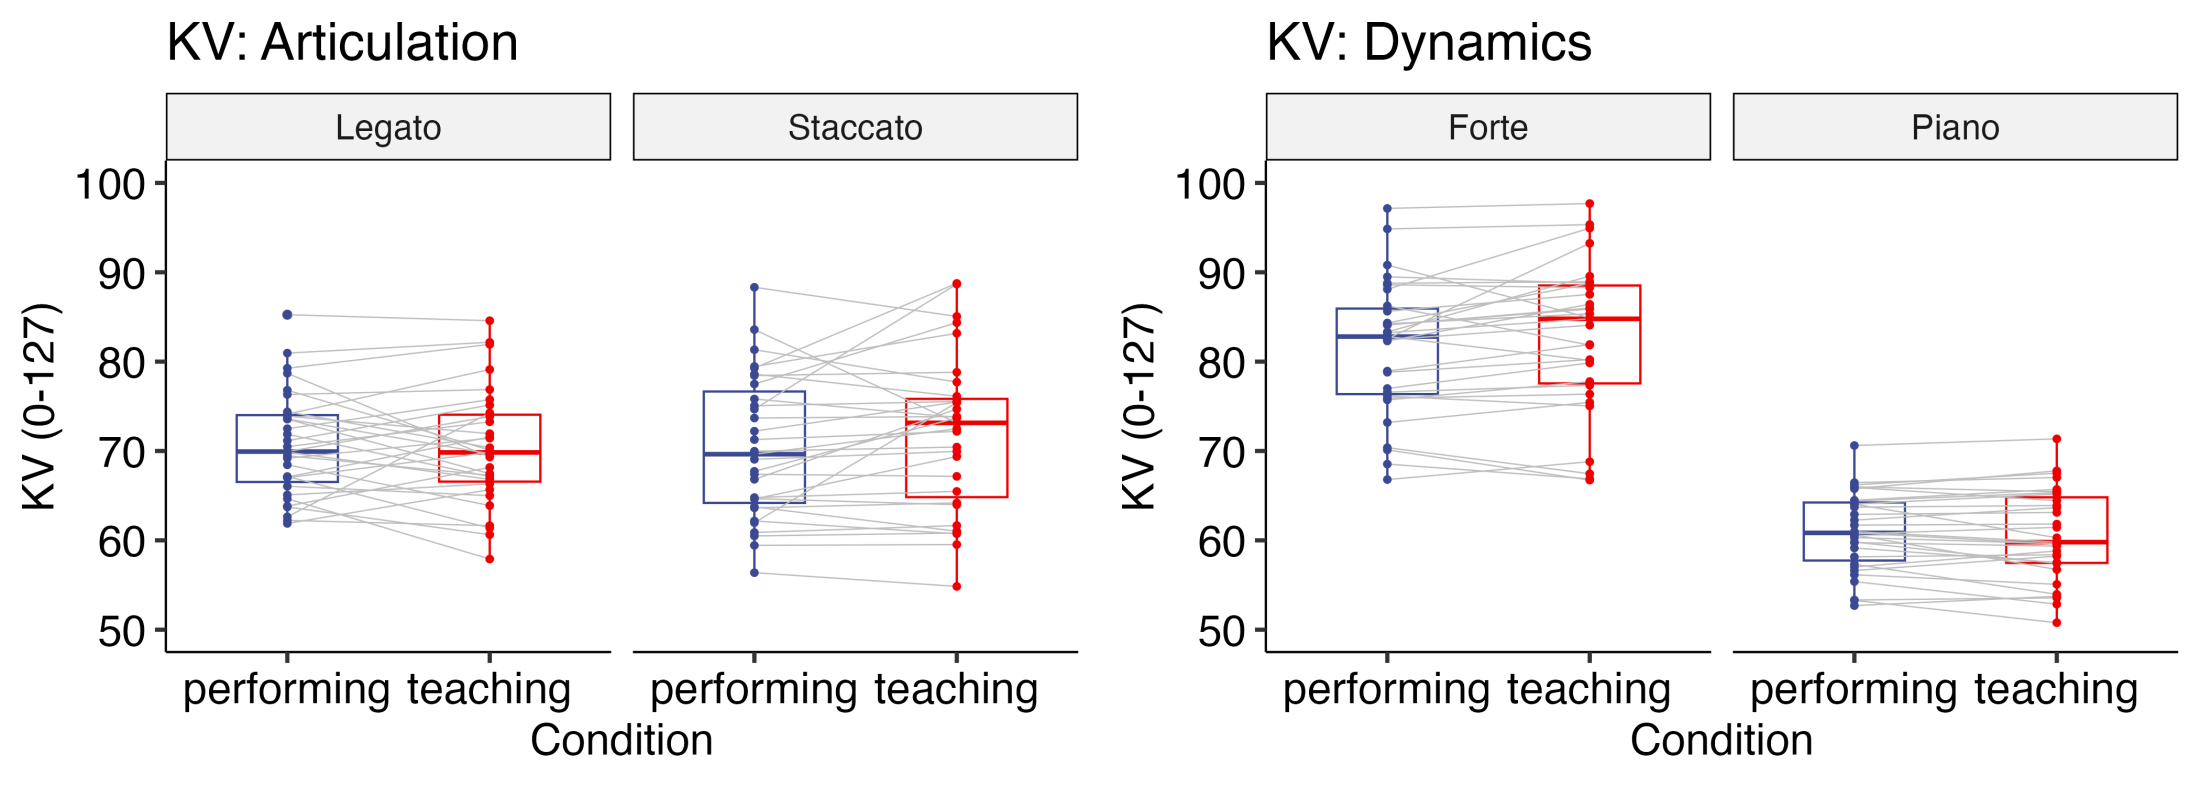
\includegraphics[width=1\linewidth]{manuscript_files/figure-latex/plot-vel-1-1} \caption{\label{fig:vel-1}Experiment 1: KV (0-127) when playing the piece with either articulation (left) or dynamics (right). Each box indicates the IQR with the median, and whiskers extend to a maximum of 1.5 × IQR beyond the box. Significance levels: * \textit{p} < .05, ** \textit{p} < .01, *** \textit{p} < .001}\label{fig:plot-vel-1}
\end{figure}

\newpage

\hypertarget{experiment-2}{%
\section{3. Experiment 2}\label{experiment-2}}

\hypertarget{method-1}{%
\subsection{3.1. Method}\label{method-1}}

\hypertarget{participants-1}{%
\subsubsection{3.1.1. Participants}\label{participants-1}}

We recruited 21 piano experts who already had a degree (above bachelor or equivalent) in piano performance/teaching or were studying advanced piano performance at a music school at the time of recruitment. For data analysis, we excluded one participant due to insufficient motor skills. Twenty participants (9 female) were included in the data analysis. Most participants were right-handed (left: 2) with a mean age of 25.90 (\emph{SD} = 4.68). They had 15.65 years of practice on average (\emph{SD} = 5.67).

\hypertarget{apparatus-and-stimuli-1}{%
\subsubsection{3.1.2. Apparatus and stimuli}\label{apparatus-and-stimuli-1}}

The same apparatus as in Experiment 1 was used. We selected Clementi's Sonatina Op.36 (No.3) in C major as a stimulus because it contained our targeted expressions (i.e., articulation, dynamics) and was relatively simple in terms of motor skills. The first 12 measures of the original piece were used and modified so that the piece had an almost equal number of data points for each dependent variable. The modified piece consisted of a 12-measure isochronous melody notated in 4/4 meter to be played with the right hand only. Non-expressive sheet music was used for the purpose of practice (\emph{Figure \ref{fig:stimuli-2}, A}). Expressive notations were added to the non-expressive sheet music for the experiment (\emph{Figure \ref{fig:stimuli-2}, B-C}). These excerpts were confirmed to be musically natural by a doctoral student in piano performance at Liszt Ferenc Academy of Music in Hungary. The fingering was also assigned and confirmed by the same doctoral student.

\hypertarget{procedure-2}{%
\subsubsection{3.1.3. Procedure}\label{procedure-2}}

We employed the same procedure as in Experiment 1 with several modifications. First, all participants were required to memorise the piece without expressive notations (i.e., \emph{Figure \ref{fig:stimuli-2}, A}) prior to the experiment. Second, we modified the wording of instructions for the performing condition so that both instructions had the same focus on expressive notations (see details in \emph{\protect\hyperlink{supplemental}{Supplementary Materials}}). Third, participants could choose their preferred tempo from one of three options (100, 110 and 120 quarter-beats per minute). The chosen tempo was again cued by a leading metronome. In order to make sure that participants memorised the piece and had sufficient motor skills, we asked participants to perform the piece without looking at the non-expressive sheet music. Those who could not perform the piece twice consecutively within five attempts were excluded from data analysis (as a result, one participant was excluded). The rest of the procedure was identical to Experiment 1.

\hypertarget{data-analysis-1}{%
\subsubsection{3.1.4. Data analysis}\label{data-analysis-1}}

Data cleaning, preprocessing and statistical analysis were almost identical to Experiment 1. For statistical analysis, only 8th notes with expressive notations were included. As a result, only one 8th note in the 4th measure without any expression was not included. IOIs were normalised by their preferred tempo because each participant chose a tempo from the three options. Given the different tempi, a key-overlap ratio (KOR) was calculated by dividing KOT by the mean IOI of each performance in order to normalise KOT. Additionally, we include KV difference (i.e., KV difference for each interval) at transition points (i.e., forte to piano or piano to forte) as a dependent variable based on the findings of Experiment 1. Three trials were entirely excluded from data analysis because participants did not follow the sheet music. Using the same approach as in Experiment 1, pitch errors were removed manually. For onsets, 11.62\% of the trials contained at least one pitch error (extra notes: 5.81\%, missing notes: 5.49\%, substituted notes: 0.31\%). For offsets, 17.90\% of the trials contained at least one pitch error (extra notes: 5.81\%, missing notes: 5.49\%, substituted notes: 6.59\%). As a result, less than 1 \% of total responses were corrected. For each dependent variable, removing outliers (i.e., responses outside 3 standard deviations from the mean) resulted in less than 5\% of overall responses being removed.

\begin{figure}
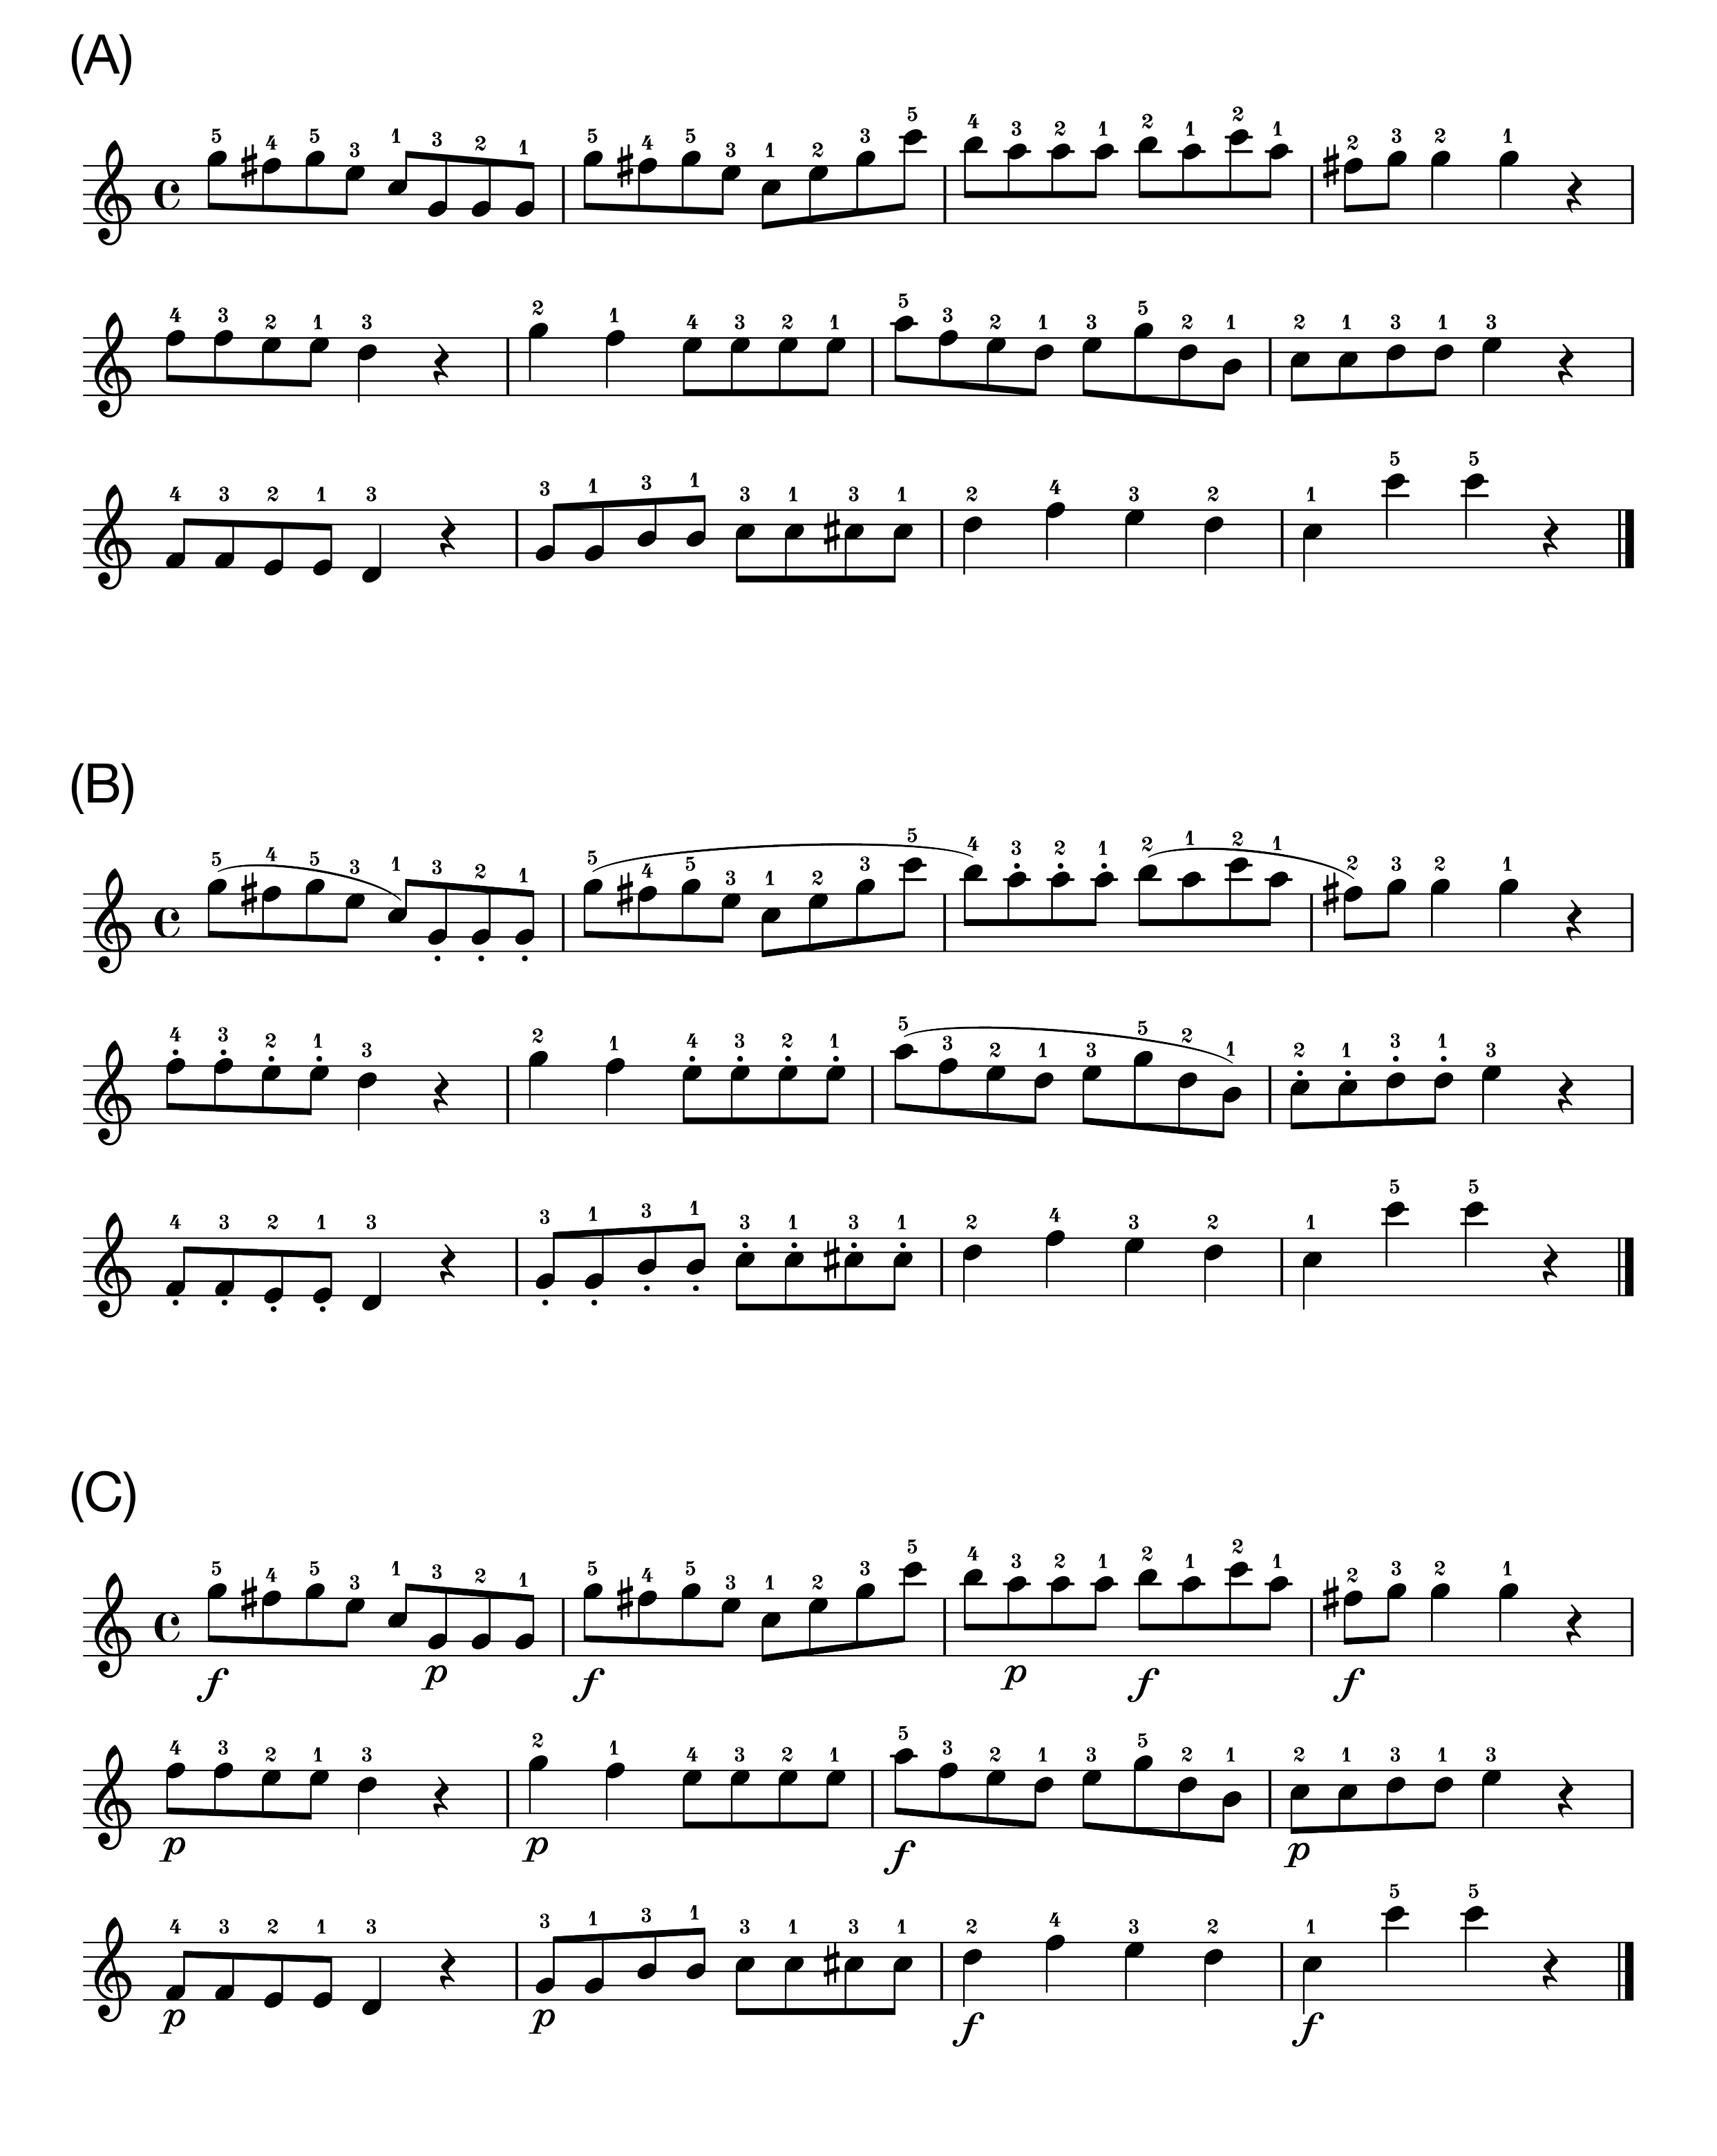
\includegraphics[width=1\linewidth]{manuscript_files/figure-latex/stim-2-1} \caption{\label{fig:stimuli-2}(A)Non-expressive sheet music. (B)Articulation. The curved line (slur) indicates legato and the dots indicate staccato. (C)Dynamics. The symbol `f' denotes forte and the symbol `p' denotes piano. For data analysis, only the 8th notes were included.}\label{fig:stim-2}
\end{figure}

\hypertarget{results-1}{%
\subsection{3.2. Results}\label{results-1}}

As Experiment 1, we first report results for performance of the piece with the notated expression of articulation (\emph{Figure \ref{fig:stimuli-2}, B}), followed by performance of the piece with the notated expression of dynamics (\emph{Figure \ref{fig:stimuli-2}, C}).

\hypertarget{articulation-interonset-intervals-iois-1}{%
\subsubsection{3.2.1. Articulation: Interonset Intervals (IOIs)}\label{articulation-interonset-intervals-iois-1}}

A paired-sample \emph{t}-test showed that participants played more slowly in the teaching condition {[}\emph{M} = 0.97, \emph{SD} = 0.049{]} than in the performing condition {[}\emph{M} = 0.95, \emph{SD} = 0.040{]} while playing the piece with the notated articulation (\emph{t}(19) = 2.47
, \emph{p} = 0.023, Cohen's \emph{d} = 0.55, \emph{Figure \ref{fig:ioi-2}}). A Wiscoxon Signed-rank test also confirmed that there was a significant difference between the two conditions (\emph{p} = 0.033, \emph{r} = 0.48).

\hypertarget{articulation-key-overlap-ratio-kor}{%
\subsubsection{3.2.2. Articulation: Key-Overlap Ratio (KOR)}\label{articulation-key-overlap-ratio-kor}}

A two-way repeated-measures ANOVA with the factors Condition (teaching vs.~performing) and Subcomponent-LS (legato vs.~staccato) showed that there was a significant main effect of Subcomponent-LS (\emph{F}(1,19) = 2573, \emph{p} \textless{} 0.001, \(\eta_G^2\) = 0.98) and a significant interaction between Condition and Subcomponent-LS (\emph{F}(1,19) = 8.91, \emph{p} = 0.008, \(\eta_G^2\) = 0.01, \emph{Figure \ref{fig:kor-2}}). Post-hoc comparisons based on the estimated marginal means with Tukey adjustment showed that participants produced shorter staccato in the teaching condition {[}\emph{M} = -0.76, \emph{SD} = 0.06{]} than in the performing condition {[}\emph{M} = -0.74, \emph{SD} = 0.04{]} (\emph{p} = 0.002) while there was no significant difference in legato between the teaching {[}\emph{M} = 0.12, \emph{SD} = 0.07{]} and performing condition {[}\emph{M} = 0.12, \emph{SD} = 0.07{]} (\emph{p} = 0.56).

\hypertarget{articulation-key-velocity-kv-1}{%
\subsubsection{3.2.3. Articulation: Key Velocity (KV)}\label{articulation-key-velocity-kv-1}}

A two-way repeated-measures ANOVA with the factors Condition (teaching vs.~performing) and Subcomponent-LS (legato vs.~staccato) showed that there was a significant main effect of Subcomponent-LS (\emph{F}(1,19) = 7.91, \emph{p} = 0.011, \(\eta_G^2\) = 0.03, \emph{Figure \ref{fig:vel-2}}), reflecting louder sound for legato notes compared to staccato notes. Neither the main effect of Condition (\emph{F}(1,19) = 1.33, \emph{p} = 0.26, \(\eta_G^2\) = 0.003) nor the interaction between Condition and Subcomponent-LS (\emph{F}(1,19) = 0.14, \emph{p} = 0.71, \(\eta_G^2\) = 0.000) was significant.

\hypertarget{dynamics-interonset-intervals-iois-1}{%
\subsubsection{3.2.4. Dynamics: Interonset Intervals (IOIs)}\label{dynamics-interonset-intervals-iois-1}}

A paired-sample \emph{t}-test showed no significant difference between the teaching condition {[}\emph{M} = 0.96, \emph{SD} = 0.048{]} and the performing condition {[}\emph{M} = 0.96, \emph{SD} = 0.043{]} while playing the piece with the notated dynamics (\emph{t}(19) = 0.21, \emph{p} = 0.84, Cohen's \emph{d} = 0.05, \emph{Figure \ref{fig:ioi-2}}). A Wiscoxon Signed-rank test also confirmed that there was no significant difference between the two conditions (\emph{p} = 0.96).

\hypertarget{dynamics-key-velocity-kv-1}{%
\subsubsection{3.2.5. Dynamics: Key Velocity (KV)}\label{dynamics-key-velocity-kv-1}}

A two-way repeated-measures ANOVA with the factors Condition (teaching vs.~performing) and Subcomponent-FP (forte vs.~piano) showed that there was a significant main effect of Subcomponent-FP (\emph{F}(1,19) = 132, \emph{p} \textless{} 0.001, \(\eta_G^2\) = 0.72) and a significant interaction between Condition and Subcomponent-FP (\emph{F}(1,19) = 6.12, \emph{p} = 0.023, \(\eta_G^2\) = 0.018, \emph{Figure \ref{fig:vel-2}}). Post-hoc comparisons based on the estimated marginal means with Tukey adjustment revealed that participants produced louder forte (\emph{p} = 0.040) and softer piano (\emph{p} = 0.024) in the teaching condition {[}Forte: \emph{M} = 83.20, \emph{SD} = 8.84, Piano: \emph{M} = 60.53, \emph{SD} = 3.76{]} than in the performing condition {[}Forte: \emph{M} = 81.49, \emph{SD} = 8.12, Piano: \emph{M} = 62.42, \emph{SD} = 4.82{]} than in the performing condition.

\hypertarget{dynamics-kv-transition-points-1}{%
\subsubsection{3.2.6. Dynamics: KV Transition Points}\label{dynamics-kv-transition-points-1}}

A two-way repeated-measures ANOVA with the factors Condition (teaching vs.~performing) and Subcomponent-FP (FtoP vs.~PtoF) showed that there was a significant main effect of Subcomponent-FP (\emph{F}(1,19) = 124, \emph{p} \textless{} 0.001, \(\eta_G^2\) = 0.82) and a significant interaction between Condition and Subcomponent-FP (\emph{F}(1,19) = 9.15, \emph{p} = 0.007, \(\eta_G^2\) = 0.059, \emph{Figure \ref{fig:vel-diff}}). Post-hoc comparisons based on the estimated marginal means with Tukey adjustment showed that there was a larger KV difference when the expressive notation changed from forte to piano (FtoP: \emph{p} = 0.029) and from piano to forte (PtoF: \emph{p} = 0.002) in the teaching condition {[}FtoP: \emph{M} = -17.23, \emph{SD} = 8.26, PtoF: \emph{M} = 20.71, \emph{SD} = 8.87{]} than in the performing condition {[}FtoP: \emph{M} = -14.04, \emph{SD} = 7.67, PtoF: \emph{M} = 16.05, \emph{SD} = 7.32{]}.

\hypertarget{dynamics-key-overlap-ratio-kor}{%
\subsubsection{3.2.7. Dynamics: Key-Overlap Ratio (KOR)}\label{dynamics-key-overlap-ratio-kor}}

A two-way repeated-measures ANOVA with the factors Condition (teaching vs.~performing) and Subcomponent-FP (forte vs.~piano) showed that there was a significant main effect of Subcomponent-FP (\emph{F}(1,19) = 630, \emph{p} \textless{} 0.001, \(\eta_G^2\) = 0.94), reflecting more key overlap for forte notes compared to piano notes. Neither the main effect of Condition (\emph{F}(1,19) = 0.081, \emph{p} = 0.78, \(\eta_G^2\) = 0.000) nor the interaction between Condition and Subcomponent-FP (\emph{F}(1,19) = 0.35, \emph{p} = 0.56, \(\eta_G^2\) = 0.001, \emph{Figure \ref{fig:kor-2}}) was significant.

\hypertarget{discussion-1}{%
\subsection{3.3. Discussion}\label{discussion-1}}

The results from Experiment 2 replicate our earlier findings and provide further evidence that skilled pianists were able to modulate their performance for teaching purposes. As in Experiment 1, we observed slower performance only while teaching the notated articulation. Again, KOR showed that when teaching articulation, participants produced shorter staccato, while there was no significant difference in legato between the two conditions. While teaching dynamics, KV showed that participants produced louder forte and softer piano. This pattern of exaggeration was more pronounced than in Experiment 1, where only louder forte was observed. Furthermore, we again found that when teaching dynamics, participants made a larger contrast between forte and piano bidirectionally at transition points. Importantly, participants did not modulate performance aspects that were irrelevant with regard to the techniques to be taught (i.e., no modulation of dynamics when teaching articulation and vice versa). Overall, Experiment 2 demonstrated systematic and fine-grained didactic performance modulations for a naturalistic piece of music.

\begin{figure}
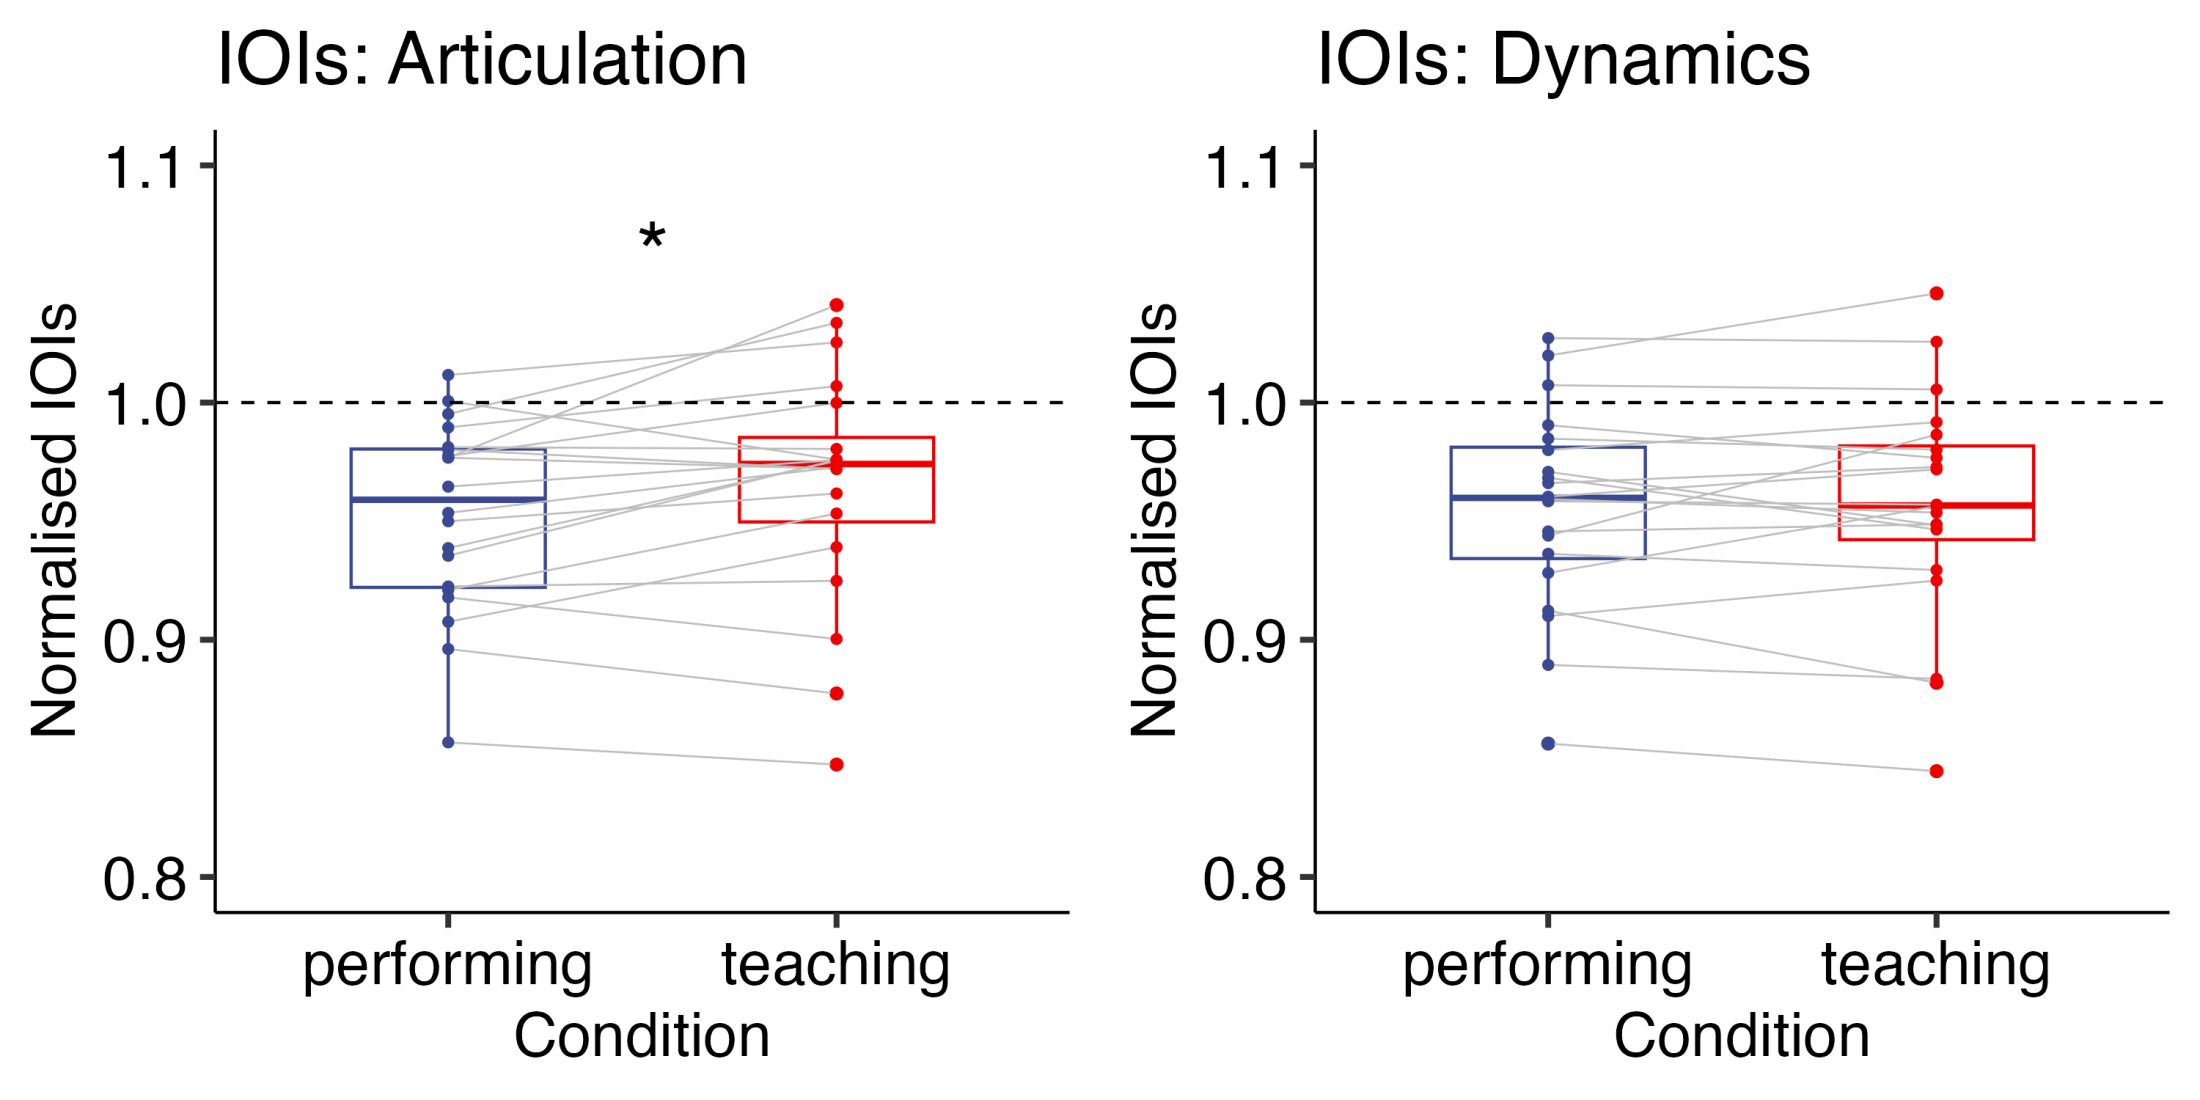
\includegraphics[width=1\linewidth]{manuscript_files/figure-latex/plot-ioi-2-1} \caption{\label{fig:ioi-2}Experiment 2: Normalised IOIs when playing the piece with either articulation (left) or dynamics (right). Each box indicates the IQR with the median, and whiskers extend to a maximum of 1.5 × IQR beyond the box. Significance levels: * \textit{p} < .05, ** \textit{p} < .01, *** \textit{p} < .001}\label{fig:plot-ioi-2}
\end{figure}

\begin{figure}
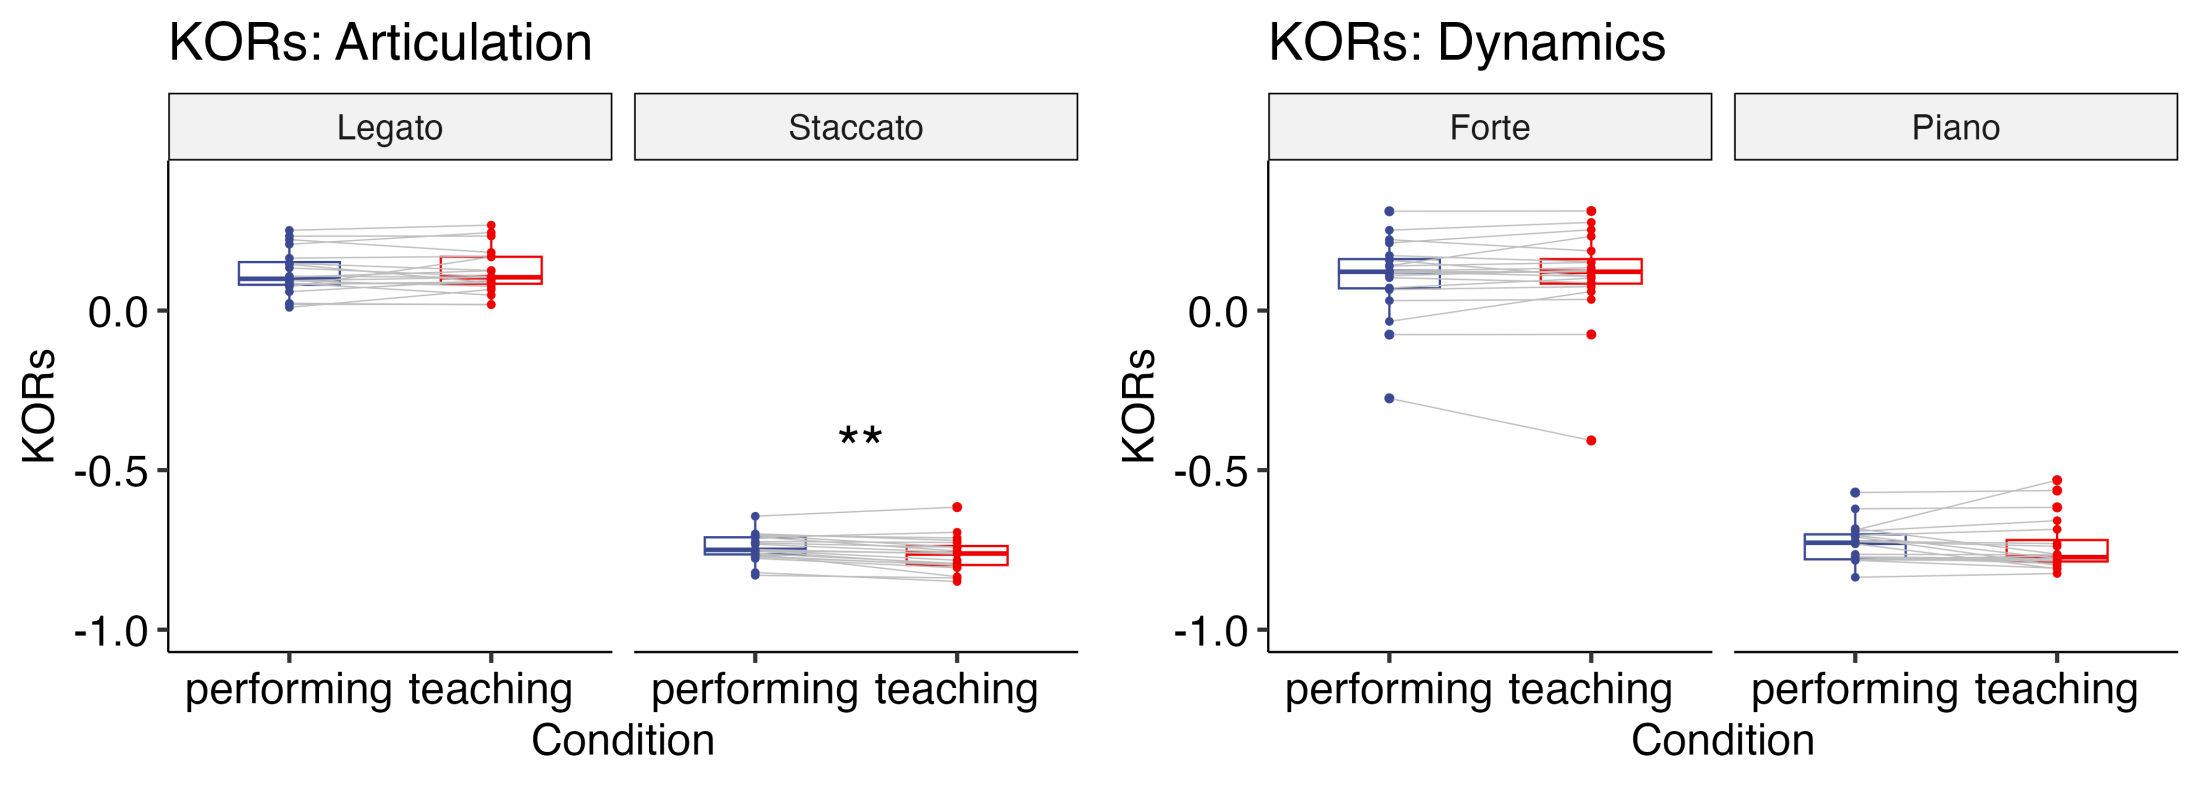
\includegraphics[width=1\linewidth]{manuscript_files/figure-latex/plot-kor-2-1} \caption{\label{fig:kor-2}Experiment 2: KOR when playing the piece with either articulation (left) or dynamics (right). Each box indicates the IQR with the median, and whiskers extend to a maximum of 1.5 × IQR beyond the box. Significance levels: * \textit{p} < .05, ** \textit{p} < .01, *** \textit{p} < .001}\label{fig:plot-kor-2}
\end{figure}

\begin{figure}
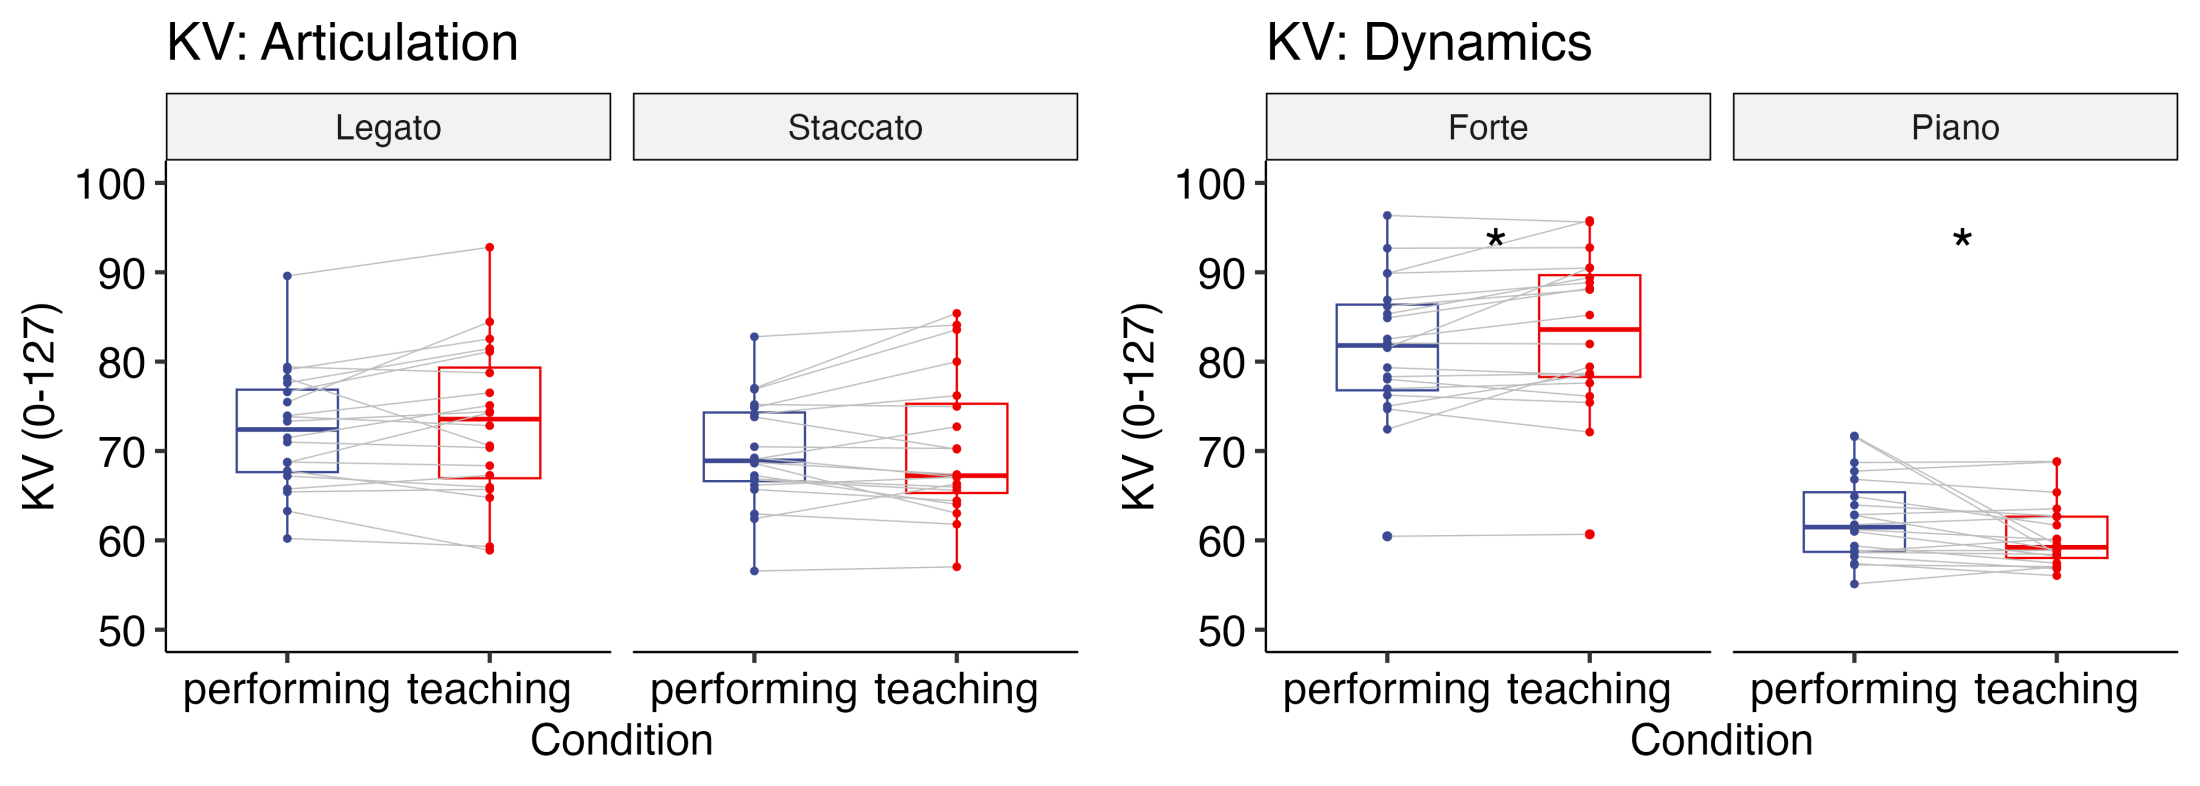
\includegraphics[width=1\linewidth]{manuscript_files/figure-latex/plot-vel-2-1} \caption{\label{fig:vel-2}Experiment 2: KV (0-127) when playing the piece with either articulation (left) or dynamics (right). Each box indicates the IQR with the median, and whiskers extend to a maximum of 1.5 × IQR beyond the box. Significance levels: * \textit{p} < .05, ** \textit{p} < .01, *** \textit{p} < .001}\label{fig:plot-vel-2}
\end{figure}

\begin{figure}
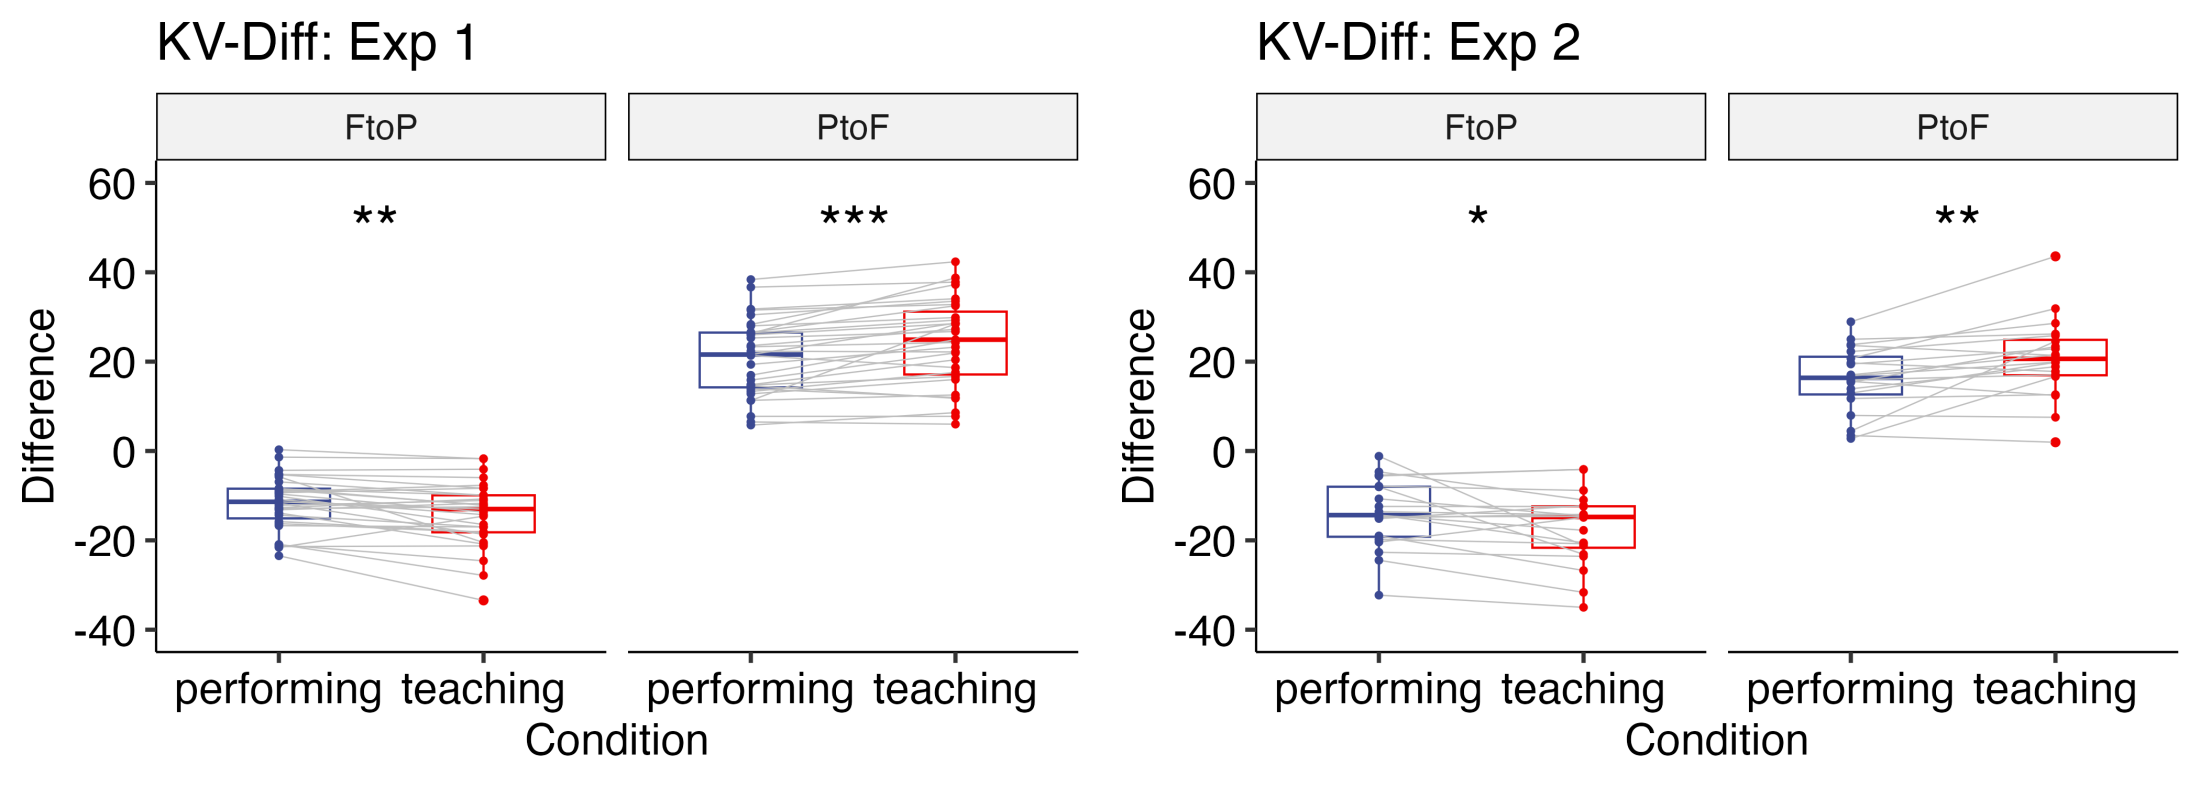
\includegraphics[width=1\linewidth]{manuscript_files/figure-latex/plot-vel-diff-1} \caption{\label{fig:vel-diff}Experiment 1, 2: KV Difference at transition points when playing the piece with dynamics (left: Experiment 1, right: Experiment 2). Each box indicates the IQR with the median, and whiskers extend to a maximum of 1.5 × IQR beyond the box. Significance levels: * \textit{p} < .05, ** \textit{p} < .01, *** \textit{p} < .001}\label{fig:plot-vel-diff}
\end{figure}

\newpage

\hypertarget{general-discussion}{%
\section{4. General Discussion}\label{general-discussion}}

The aim of the study was to investigate how expert pianists modulate their performance in order to teach expressive techniques. Overall, the findings of the two experiments showed that pianists performed one and the same piece differently depending on whether they played with the intention to teach expressive techniques or with the intention to perform the piece for an audience. When playing with the intention to teach, pianists selectively highlighted relevant aspects of artistic expressions. Across two different pieces, they exaggerated staccato when playing with the intention to teach expressions concerning articulation. The lack of a difference for legato when teaching articulation might stem from a ceiling effect. When playing with the intention to teach expressions concerning dynamics, participants exaggerated changes between forte and piano (in both directions). This constitutes an effective way to highlight the technique as loudness is determined relatively. Taken together, our findings demonstrate that expert pianists systematically modulated their sound depending on the specific technique they were trying to convey.

Although participants tended to play slower in the teaching condition than in the performing condition in general, we found a significant difference only for articulation, not for dynamics. As mentioned in the discussion of Experiment 1, it could be that the metronome beats given prior to each performance discouraged participants from deviating from the prescribed tempo. Another possibility is that expression is actually best taught when leaving the tempo unchanged when it is irrelevant. This would imply that general didactic modulations like slowing down might be less useful in the context of teaching expressive techniques where timing itself can be used to add an expression to a performance.

Musicians and music teachers tend to consider expressive skills as a performer's most important skill (Lindström, Juslin, Bresin, \& Williamon, 2003). In the present study, experts focused on the teaching of expressions that were notated. However, expression also has other facets (Juslin, 2003) that are not only piece-related but performer- or context-related. An interesting topic for future research is how experts teach not only expressive techniques as such but convey possibilities of interpretation.

One limitation of the study is that although we instructed participants to imagine a situation in which they were teaching musical expression to students, there was no feedback from actual students. Given that teachers modulate their demonstration throughout online interactions with learners (Okazaki, Muraoka, \& Osu, 2019), future studies are needed to investigate how experts dynamically adapt their performance to their students' skill level and demonstrated abilities.

The present findings extend earlier research on teaching-related action modulations. First, our study sheds light on the teaching of expressive techniques that are an integral part of skill acquisition in artistic domains. We showed that compared to an expressive performance baseline, experts made specific modulations in order to teach particular techniques. Second, the specificity of the observed modulations supports the idea that teaching comprises more than generic modulations like slowing down or overall exaggeration that may draw learners' attention. Rather, expert demonstrators seem to follow principles of relevance in communication (Sperber \& Wilson, 1995), highlighting only those aspects they are intending to demonstrate. How learners benefit from the perceptual and motor cues that come with specific exaggerations, and whether understanding the teacher's intentions explicitly adds to the learning success are important questions for future research.

\hypertarget{acknowledgements}{%
\section{Acknowledgements}\label{acknowledgements}}

We thank Dávid Csűrös for his help with data collection. This research was supported by the European Research Council under the European Union's Seventh Framework Program (FP7/2007-2013)/ERC (European Research Council) grant agreement no. 609819, SOMICS, and by ERC grant agreement no. 616072, JAXPERTISE.

\hypertarget{declarations-of-interest}{%
\section{Declarations of interest}\label{declarations-of-interest}}

The authors have no conflict of interest.

\newpage

\hypertarget{references}{%
\section{References}\label{references}}

\begingroup
\setlength{\parindent}{-0in}
\setlength{\leftskip}{0in}

\hypertarget{refs}{}
\begin{CSLReferences}{1}{0}
\leavevmode\vadjust pre{\hypertarget{ref-brand_2002}{}}%
Brand, R. J., Baldwin, D. A., \& Ashburn, L. A. (2002). Evidence for {`motionese'}: Modifications in mothers' infant-directed action. \emph{Developmental Science}, \emph{5}(1), 72--83. \url{https://doi.org/10.1111/1467-7687.00211}

\leavevmode\vadjust pre{\hypertarget{ref-bresin_2000}{}}%
Bresin, R., \& Battel, G. U. (2000). Articulation {Strategies} in {Expressive Piano Performance Analysis} of {Legato}, {Staccato}, and {Repeated Notes} in {Performances} of the {Andante Movement} of {Mozart}'s {Sonata} in {G Major} ({K} 545). \emph{Journal of New Music Research}, \emph{29}(3), 211--224. \url{https://doi.org/10.1076/jnmr.29.3.211.3092}

\leavevmode\vadjust pre{\hypertarget{ref-campisi_2013}{}}%
Campisi, E., \& Özyürek, A. (2013). Iconicity as a communicative strategy: {Recipient} design in multimodal demonstrations for adults and children. \emph{Journal of Pragmatics}, \emph{47}(1), 14--27. \url{https://doi.org/10.1016/j.pragma.2012.12.007}

\leavevmode\vadjust pre{\hypertarget{ref-csibra_2009}{}}%
Csibra, G., \& Gergely, G. (2009). Natural pedagogy. \emph{Trends in Cognitive Sciences}, \emph{13}(4), 148--153. \url{https://doi.org/10.1016/j.tics.2009.01.005}

\leavevmode\vadjust pre{\hypertarget{ref-fukuyama_2015}{}}%
Fukuyama, H., Qin, S., Kanakogi, Y., Nagai, Y., Asada, M., \& Myowa-Yamakoshi, M. (2015). Infant's action skill dynamically modulates parental action demonstration in the dyadic interaction. \emph{Developmental Science}, \emph{18}(6), 1006--1013. \url{https://doi.org/10.1111/desc.12270}

\leavevmode\vadjust pre{\hypertarget{ref-NIPS2016_6413}{}}%
Ho, M. K., Littman, M., MacGlashan, J., Cushman, F., \& Austerweil, J. L. (2016). Showing versus doing: {Teaching} by demonstration. In D. D. Lee, M. Sugiyama, U. V. Luxburg, I. Guyon, \& R. Garnett (Eds.), \emph{Advances in neural information processing systems 29} (pp. 3027--3035). {Curran Associates, Inc.}

\leavevmode\vadjust pre{\hypertarget{ref-juslin_2003}{}}%
Juslin, P. N. (2003). Five {Facets} of {Musical Expression}: {A Psychologist}'s {Perspective} on {Music Performance}. \emph{Psychology of Music}, \emph{31}(3), 273--302. \url{https://doi.org/10.1177/03057356030313003}

\leavevmode\vadjust pre{\hypertarget{ref-lindstrom_2003}{}}%
Lindström, E., Juslin, P. N., Bresin, R., \& Williamon, A. (2003). {``{Expressivity} comes from within your soul''}: {A} questionnaire study of music students' perspectives on expressivity. \emph{Research Studies in Music Education}, \emph{20}(1), 23--47. \url{https://doi.org/10.1177/1321103X030200010201}

\leavevmode\vadjust pre{\hypertarget{ref-mcellin_2017}{}}%
McEllin, L., Knoblich, G., \& Sebanz, N. (2017). Distinct kinematic markers of demonstration and joint action coordination? {Evidence} from virtual xylophone playing. \emph{Journal of Experimental Psychology: Human Perception and Performance}, \emph{44}(6), 885. \url{https://doi.org/10.1037/xhp0000505}

\leavevmode\vadjust pre{\hypertarget{ref-okazaki_2019}{}}%
Okazaki, S., Muraoka, Y., \& Osu, R. (2019). Teacher-learner interaction quantifies scaffolding behaviour in imitation learning. \emph{Sci Rep}, \emph{9}(1), 1--13. \url{https://doi.org/10.1038/s41598-019-44049-x}

\leavevmode\vadjust pre{\hypertarget{ref-saint-georges_2013}{}}%
Saint-Georges, C., Chetouani, M., Cassel, R., Apicella, F., Mahdhaoui, A., Muratori, F., \ldots{} Cohen, D. (2013). Motherese in {Interaction}: {At} the {Cross}-{Road} of {Emotion} and {Cognition}? ({A Systematic Review}). \emph{PLOS ONE}, \emph{8}(10), e78103. \url{https://doi.org/10.1371/journal.pone.0078103}

\leavevmode\vadjust pre{\hypertarget{ref-schaik_2019}{}}%
Schaik, J. E. van, Meyer, M., Ham, C. R. van, \& Hunnius, S. (2019). Motion tracking of parents' infant- versus adult-directed actions reveals general and action-specific modulations. \emph{Developmental Science}, \emph{0}(0), e12869. \url{https://doi.org/10.1111/desc.12869}

\leavevmode\vadjust pre{\hypertarget{ref-sloboda_2000}{}}%
Sloboda, J. A. (2000). Individual differences in music performance. \emph{Trends in Cognitive Sciences}, \emph{4}(10), 397--403. \url{https://doi.org/10.1016/S1364-6613(00)01531-X}

\leavevmode\vadjust pre{\hypertarget{ref-sperber_1995}{}}%
Sperber, D., \& Wilson, D. (1995). \emph{Relevance: {Communication} and cognition, 2nd ed}. {Malden}: {Blackwell Publishing}.

\leavevmode\vadjust pre{\hypertarget{ref-thornton_2008}{}}%
Thornton, A., \& Raihani, N. J. (2008). The evolution of teaching. \emph{Animal Behaviour}, \emph{75}(6), 1823--1836. \url{https://doi.org/10.1016/j.anbehav.2007.12.014}

\leavevmode\vadjust pre{\hypertarget{ref-tomasello_2016}{}}%
Tomasello, M. (2016). The ontogeny of cultural learning. \emph{Current Opinion in Psychology}, \emph{8}, 1--4. \url{https://doi.org/10.1016/j.copsyc.2015.09.008}

\leavevmode\vadjust pre{\hypertarget{ref-uther_2007}{}}%
Uther, M., Knoll, M. A., \& Burnham, D. (2007). Do you speak {E}-{NG}-{L}-{I}-{SH}? {A} comparison of foreigner- and infant-directed speech. \emph{Speech Communication}, \emph{49}(1), 2--7. \url{https://doi.org/10.1016/j.specom.2006.10.003}

\end{CSLReferences}

\endgroup

\clearpage

\hypertarget{supplementary}{%
\section{Supplementary Materials}\label{supplementary}}

\hypertarget{instructions}{%
\subsection{Instructions}\label{instructions}}

\hypertarget{experiment-1-1}{%
\subsubsection{Experiment 1}\label{experiment-1-1}}

In the teaching condition, participants were shown the following instruction on a computer monitor (Italic sentences were highlighted in yellow colour on a black background): ``Now, play what you practised as if you were teaching it to students. Students already know how to produce the sequence of the tones and now are trying to \emph{learn how to perform the piece expressively} by listening to your performance. \emph{Do your best as a teacher to produce the piece according to the notation that you just practised.}''

In the performing condition, participants were shown the following instruction on a computer monitor monitor: ``Now, play what you practised as if you were performing it to an audience. \emph{Do your best as a performer to produce the piece according to the notation that you just practised.}''

\hypertarget{experiment-2-1}{%
\subsubsection{Experiment 2}\label{experiment-2-1}}

In the teaching condition of Experiment 2, we gave participants the exact same instruction as in Experiment 1. In the performing condition, participants were given the following instruction on a computer monitor: ``Now, play what you practised as if you were performing it to an audience. \emph{Perform the piece expressively with your interpretation. Do your best as a performer to produce the piece according to the notation that you just practised.}''


\end{document}
